\documentclass[11pt,a4paper]{article}

% Image mode: pdf.
% Image paths stay relative. In PDF mode, place same-basename PDF conversions
% of the chapter SVG files in the assets/ directory beside this source.

\usepackage{iftex}
\ifPDFTeX
  \PackageError{handout}{This template requires XeTeX or Tectonic}{Compile with xelatex or tectonic.}
\fi

\usepackage[a4paper,top=18mm,bottom=20mm,left=20mm,right=20mm,headsep=6mm]{geometry}
\usepackage{fontspec}
\usepackage{xeCJK}
\usepackage{amsmath}
\usepackage{unicode-math}

% Font settings are intentionally visible in the generated .tex file.
% These defaults target the macOS machine used for the released PDF.
% Change the family names when compiling on another system.
\setmainfont{Songti TC}
\setsansfont{Heiti TC}
\setmonofont{Menlo}
\setCJKmainfont{Songti TC}
\setCJKsansfont{Heiti TC}
\setCJKmonofont{Heiti TC}
\setmathfont{STIX Two Math}
\XeTeXlinebreaklocale "zh"
\XeTeXlinebreakskip=0pt plus 1pt

\usepackage{xcolor}
\definecolor{HandoutBlue}{HTML}{215A91}
\definecolor{HandoutBlueLight}{HTML}{EEF5FC}
\definecolor{HandoutGreen}{HTML}{39715A}
\definecolor{HandoutGreenLight}{HTML}{EFF8F3}
\definecolor{HandoutGold}{HTML}{8A641C}
\definecolor{HandoutGoldLight}{HTML}{FFF8E8}
\definecolor{HandoutInk}{HTML}{253142}
\definecolor{HandoutMuted}{HTML}{667085}

\usepackage{graphicx}
\makeatletter
% Pandoc 3 emits an accessibility `alt` key for raster/PDF images. Older
% graphicx releases do not know that key, so accept it without changing layout.
\@ifundefined{KV@Gin@alt}{\define@key{Gin}{alt}{}}{}
\newsavebox\pandoc@box
\newcommand*\pandocbounded[1]{%
  \sbox\pandoc@box{#1}%
  \Gscale@div\@tempa{\textheight}{\dimexpr\ht\pandoc@box+\dp\pandoc@box\relax}%
  \Gscale@div\@tempb{\linewidth}{\wd\pandoc@box}%
  \ifdim\@tempb\p@<\@tempa\p@\let\@tempa\@tempb\fi
  \ifdim\@tempa\p@<\p@\scalebox{\@tempa}{\usebox\pandoc@box}%
  \else\usebox{\pandoc@box}%
  \fi
}
\makeatother
\usepackage{float}
\floatplacement{figure}{H}
% Pandoc uses LTcaptype=none for uncaptioned longtables. The caption package
% expects that name to exist as a counter even though it is never displayed.
\newcounter{none}
\usepackage{caption}
\captionsetup[figure]{labelformat=empty,labelsep=none,font=small}

\usepackage{booktabs,longtable,array,calc}
\usepackage{etoolbox}
\makeatletter
\patchcmd\longtable{\par}{\if@noskipsec\mbox{}\fi\par}{}{}
\makeatother

\usepackage[most]{tcolorbox}
\tcbuselibrary{breakable,skins}
\newtcolorbox{HandoutLearningMap}{
  enhanced,breakable,colback=HandoutBlueLight,colframe=HandoutBlue,
  boxrule=0.8pt,arc=1.5mm,left=3mm,right=3mm,top=2mm,bottom=2mm,
  before skip=8pt,after skip=10pt
}
\newtcolorbox{HandoutWorkedExample}{
  enhanced,breakable,colback=HandoutGreenLight,colframe=HandoutGreen,
  boxrule=0.65pt,arc=1.5mm,left=3mm,right=3mm,top=2mm,bottom=2mm,
  before skip=8pt,after skip=10pt
}
\newtcolorbox{HandoutSelfCheck}{
  enhanced,breakable,colback=HandoutGoldLight,colframe=HandoutGold,
  boxrule=0.65pt,arc=1.5mm,left=3mm,right=3mm,top=2mm,bottom=2mm,
  before skip=8pt,after skip=10pt
}

\usepackage{titlesec}
\titleformat{\section}{\sffamily\bfseries\Large\color{HandoutBlue}}{}{0pt}{}
\titleformat{\subsection}{\sffamily\bfseries\large\color{HandoutInk}}{}{0pt}{}
\titleformat{\subsubsection}{\sffamily\bfseries\normalsize\color{HandoutInk}}{}{0pt}{}
\titlespacing*{\section}{0pt}{1.4em}{0.55em}
\titlespacing*{\subsection}{0pt}{1.15em}{0.45em}
\titlespacing*{\subsubsection}{0pt}{0.9em}{0.35em}
\setcounter{secnumdepth}{-\maxdimen}

\usepackage{hyperref}
\usepackage{bookmark}
\IfFileExists{xurl.sty}{\usepackage{xurl}}{}
\urlstyle{same}
\hypersetup{
  colorlinks=true,
  linkcolor=HandoutBlue,
  urlcolor=HandoutBlue,
  citecolor=HandoutBlue,
  pdftitle={數B3-3 平面向量與應用},
  pdfsubject={數學},
  pdfcreator={Pandoc with the HighSchooContent LaTeX template}
}

\setlength{\parindent}{0pt}
\setlength{\parskip}{0.55em plus 0.15em minus 0.1em}
\setlength{\emergencystretch}{3em}
\setlength{\LTpre}{0.5em}
\setlength{\LTpost}{0.5em}
\renewcommand{\arraystretch}{1.18}
\providecommand{\tightlist}{%
  \setlength{\itemsep}{0pt}\setlength{\parskip}{0pt}}
\pagestyle{plain}


\begin{document}

\begin{tcolorbox}[
  enhanced,colback=white,colframe=HandoutBlue,boxrule=1.1pt,arc=2mm,
  borderline west={3pt}{0pt}{HandoutBlue},left=5mm,right=4mm,top=4mm,bottom=4mm
]
{\sffamily\small\bfseries\color{HandoutBlue}學生講義}\par
{\sffamily\bfseries\LARGE\color{HandoutInk}數B3-3 平面向量與應用}\par
\vspace{0.35em}{\large 用大小與方向統一處理位移、比例、投影、直線、透視與平面設計}\par
\vspace{0.45em}{\small\color{HandoutMuted}%
科目：數學
\quad 課程：普通高中數學B 第三冊
\quad 版本：學生版｜核心＋理解
\quad 校訂：2026-08-29
}\par
\vspace{0.25em}{\small\color{HandoutMuted}範圍：114 學年度數學B第三冊第 3 章；平面向量表示與運算、線性組合、分點、內積、正射影、法向量、單點透視、紙張比例、黃金比例與圓角設計}\par
\end{tcolorbox}


\begin{HandoutLearningMap}

\subsection{本章問題與能力}\label{ux672cux7ae0ux554fux984cux8207ux80fdux529b}

\begin{enumerate}
\def\labelenumi{\arabic{enumi}.}
\tightlist
\item
  如何同時記錄一段移動的大小與方向，並把多段移動合成？
\item
  如何以兩個基準方向定位平面上的點，計算內分點與外分點？
\item
  如何由內積求夾角、功、正射影、點到直線的距離與直線夾角？
\item
  透視圖中的長度為何隨深度縮短，消失點與相似三角形如何決定比例？
\item
  A 系列紙張、黃金分割與圓角設計中的比例如何由方程與幾何條件得到？
\end{enumerate}

本章路徑：向量幾何 → 坐標與線性組合 → 分點與圖形變換 → 內積 → 正射影與法向量 → 透視與比例設計。

\end{HandoutLearningMap}

\section{0. 本章用途與模型範圍}\label{ux672cux7ae0ux7528ux9014ux8207ux6a21ux578bux7bc4ux570d}

位移、速度與力都同時包含大小與方向。向量把這兩項資訊保留在同一個量中，因此可以合成船速與水流、從兩次位置觀測推算移動軌跡，也可以把平面圖形縮放、平移或分割。

內積把兩個方向轉成一個數。它量出一個向量沿另一方向的有效分量，直接連到力所作的功、正射影、垂直判定、點到直線距離與兩直線夾角。坐標運算提供精確結果，幾何圖則負責確認方向與位置。

單點透視把三維場景投到平面。深度方向的平行線在圖上通向同一個消失點，物體尺寸依觀察距離的相似比縮放。紙張與平面設計則用相似、面積倍率、切線與弧長維持可重複的規格。這些高中模型處理理想化的直線投影與平面幾何；鏡頭畸變、材料裁切誤差與完整三維繪圖需要額外校正。

\section{1. 向量的幾何表示與運算}\label{ux5411ux91cfux7684ux5e7eux4f55ux8868ux793aux8207ux904bux7b97}

\subsection{1.1 定義、大小與方向}\label{ux5b9aux7fa9ux5927ux5c0fux8207ux65b9ux5411}

從點 \(A\) 指向點 \(B\) 的有向線段記為 \(\overrightarrow{AB}\)。它代表一個\textbf{向量}，包含大小 \(|\overrightarrow{AB}|=AB\) 與由 \(A\) 指向 \(B\) 的方向。

兩向量大小相等且方向相同時稱為\textbf{相等向量}。向量可平行搬移，所以起點位置不影響向量本身。大小為 \(0\) 的向量稱為\textbf{零向量} \(\vec 0\)；它的起點與終點重合。

\begin{figure}
\centering
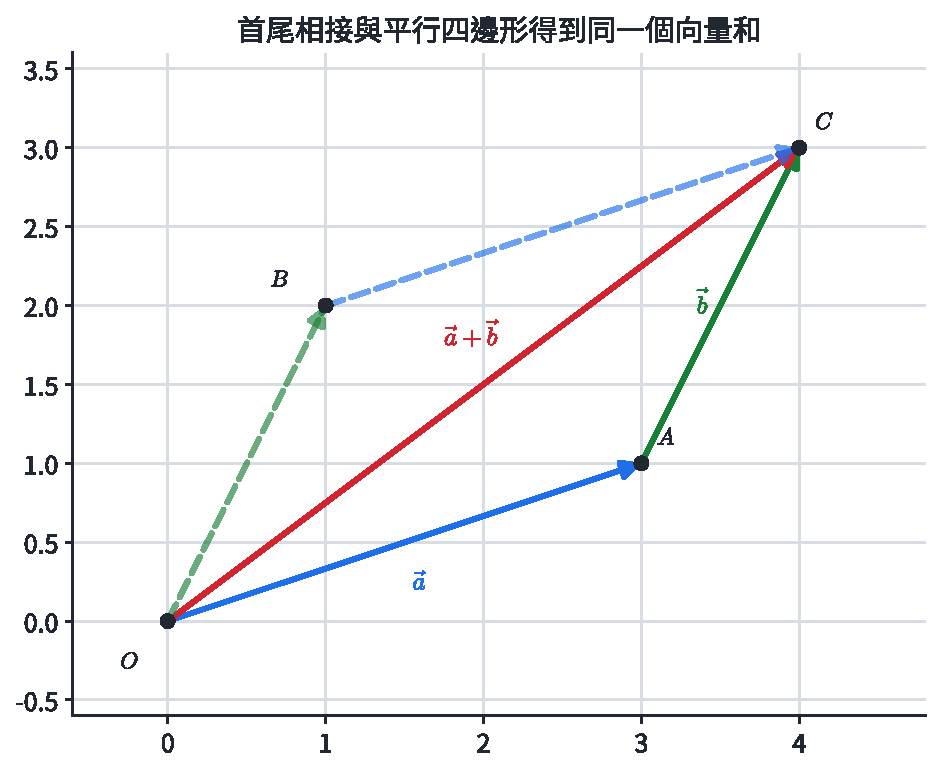
\includegraphics[width=0.88\linewidth,height=\textheight,keepaspectratio,alt={向量加減與平移}]{assets/數B3-3-向量加減與平移.pdf}
\caption{向量加減與平移}
\end{figure}

圖中藍色 \(\vec a\) 後接綠色 \(\vec b\)，從共同起點直接指向終點的紅色向量為 \(\vec a+\vec b\)。這是三角形法則：

\[
\overrightarrow{AB}+\overrightarrow{BC}=\overrightarrow{AC}.
\]

相反向量 \(-\vec b\) 與 \(\vec b\) 大小相同、方向相反，因此 \(\vec a-\vec b=\vec a+(-\vec b)\)。實數 \(k\) 與向量 \(\vec a\) 的積滿足 \(|k\vec a|=|k|\,|\vec a|\)；\(k>0\) 時同向，\(k<0\) 時反向，\(k=0\) 時為零向量。

\subsection{示範 1｜用端點消去化簡向量}\label{ux793aux7bc4-1ux7528ux7aefux9edeux6d88ux53bbux5316ux7c21ux5411ux91cf}

化簡 \(\overrightarrow{AB}+\overrightarrow{CD}+\overrightarrow{BC}\)。

\textbf{解。} 向量加法可交換次序：

\[
\overrightarrow{AB}+\overrightarrow{BC}+\overrightarrow{CD}
=\overrightarrow{AC}+\overrightarrow{CD}=\overrightarrow{AD}.
\]

每次都讓前一段終點接到下一段起點，結果是整段位移。

\subsection{示範 2｜船速與水流的合成}\label{ux793aux7bc4-2ux8239ux901fux8207ux6c34ux6d41ux7684ux5408ux6210}

船相對水面的速度為向北 \(12\text{ m/s}\)，水流向東 \(5\text{ m/s}\)。求船相對河岸的速率與方向。

\textbf{解。} 取東為 \(x\) 正向、北為 \(y\) 正向，合速度分量為 \((5,12)\)：

\[
|\vec v|=\sqrt{5^2+12^2}=13\text{ m/s}.
\]

若方向寫成北偏東 \(\theta\)，則 \(\tan\theta=5/12\)，所以 \(\theta\approx22.6^\circ\)。

\subsection{1.2 分節練習}\label{ux5206ux7bc0ux7df4ux7fd2}

\begin{enumerate}
\def\labelenumi{\arabic{enumi}.}
\tightlist
\item
  化簡 \(\overrightarrow{PQ}+\overrightarrow{RS}+\overrightarrow{QR}\)。
\item
  已知 \(|\vec a|=4\)，寫出 \(|-3\vec a|\)，並敘述方向。
\item
  正六邊形 \(ABCDEF\) 中，化簡 \(\overrightarrow{AB}+\overrightarrow{BC}+\overrightarrow{CD}\)。
\item
  無風時飛機向東速率 \(240\text{ km/h}\)，風向北、速率 \(70\text{ km/h}\)。求地速大小與方向。
\end{enumerate}

\subsection{1.3 分節練習解析}\label{ux5206ux7bc0ux7df4ux7fd2ux89e3ux6790}

\begin{enumerate}
\def\labelenumi{\arabic{enumi}.}
\tightlist
\item
  \(\overrightarrow{PQ}+\overrightarrow{QR}+\overrightarrow{RS}=\overrightarrow{PS}\)。
\item
  \(|-3\vec a|=3|\vec a|=12\)；方向與 \(\vec a\) 相反。
\item
  依序首尾相接，結果為 \(\overrightarrow{AD}\)。
\item
  地速分量為 \((240,70)\)，大小 \(250\text{ km/h}\)；方向東偏北 \(\tan^{-1}(70/240)\approx16.3^\circ\)。
\end{enumerate}

\section{2. 向量的坐標表示與平行判定}\label{ux5411ux91cfux7684ux5750ux6a19ux8868ux793aux8207ux5e73ux884cux5224ux5b9a}

\subsection{2.1 位置向量與分量}\label{ux4f4dux7f6eux5411ux91cfux8207ux5206ux91cf}

點 \(P(x,y)\) 的\textbf{位置向量}是 \(\overrightarrow{OP}=(x,y)\)。若 \(A(x_1,y_1)\)、\(B(x_2,y_2)\)，則

\[
\overrightarrow{AB}=\overrightarrow{OB}-\overrightarrow{OA}
=(x_2-x_1,\ y_2-y_1).
\]

\begin{figure}
\centering
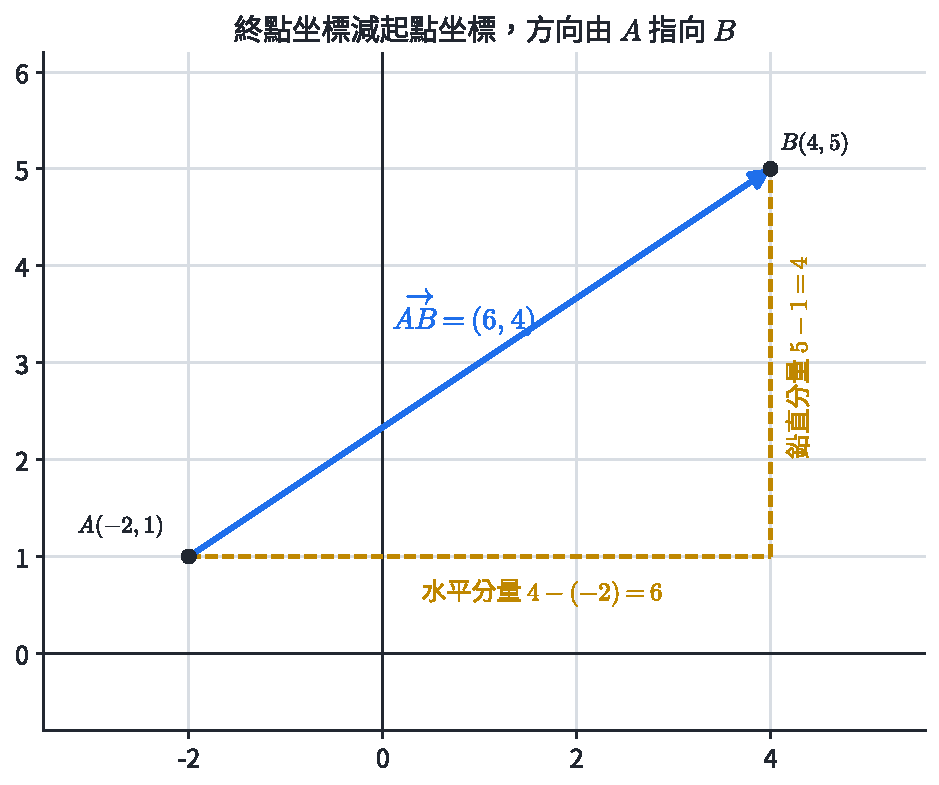
\includegraphics[width=0.88\linewidth,height=\textheight,keepaspectratio,alt={坐標向量由終點減起點}]{assets/數B3-3-坐標向量.pdf}
\caption{坐標向量由終點減起點}
\end{figure}

圖中的水平與鉛直分量分別是 \(6\) 與 \(4\)，所以 \(\overrightarrow{AB}=(6,4)\)。向量長度與坐標運算為

\[
|(u,v)|=\sqrt{u^2+v^2},
\]

\[
(a,b)+(c,d)=(a+c,b+d),\qquad k(a,b)=(ka,kb).
\]

兩個非零向量 \(\vec a,\vec b\) 平行的充要條件是存在非零實數 \(r\)，使 \(\vec b=r\vec a\)。若 \(\vec a=(a_1,a_2)\)、\(\vec b=(b_1,b_2)\)，也可使用

\[
a_1b_2-a_2b_1=0.
\]

\subsection{示範 1｜由兩點求向量與長度}\label{ux793aux7bc4-1ux7531ux5169ux9edeux6c42ux5411ux91cfux8207ux9577ux5ea6}

已知 \(A(-3,2)\)、\(B(5,-4)\)，求 \(\overrightarrow{AB}\) 與 \(AB\)。

\textbf{解。}

\[
\overrightarrow{AB}=(5-(-3),-4-2)=(8,-6),
\]

\[
AB=\sqrt{8^2+(-6)^2}=10.
\]

\subsection{示範 2｜以平行條件求參數}\label{ux793aux7bc4-2ux4ee5ux5e73ux884cux689dux4ef6ux6c42ux53c3ux6578}

已知 \(\vec a=(2,-3)\)、\(\vec b=(k,12)\) 平行，求 \(k\)。

\textbf{解。}

\[
2\cdot12-(-3)k=0\Rightarrow24+3k=0\Rightarrow k=-8.
\]

此時 \(\vec b=-4\vec a\)，方向相反且互相平行。

\subsection{2.2 分節練習}\label{ux5206ux7bc0ux7df4ux7fd2-1}

\begin{enumerate}
\def\labelenumi{\arabic{enumi}.}
\tightlist
\item
  \(A(4,-1)\)、\(B(-2,7)\)，求 \(\overrightarrow{AB}\) 與 \(AB\)。
\item
  求 \(3(2,-1)-2(-4,5)\)。
\item
  已知 \((m,6)\) 與 \((2,-3)\) 平行，求 \(m\)。
\item
  隕石在 8:00 位於 \((-5,4)\)，8:30 位於 \((-2,2)\)，保持等速度直線移動。求撞到 \(y=0\) 的時間與位置。
\end{enumerate}

\subsection{2.3 分節練習解析}\label{ux5206ux7bc0ux7df4ux7fd2ux89e3ux6790-1}

\begin{enumerate}
\def\labelenumi{\arabic{enumi}.}
\tightlist
\item
  \(\overrightarrow{AB}=(-6,8)\)，\(AB=10\)。
\item
  \((6,-3)-(-8,10)=(14,-13)\)。
\item
  \(m(-3)-6(2)=0\)，得 \(m=-4\)。
\item
  每 30 分鐘位移 \((3,-2)\)。從 \(y=4\) 降到 \(0\) 需兩段，共 \(60\) 分鐘；位置為 \((-5,4)+2(3,-2)=(1,0)\)，時間 9:00。
\end{enumerate}

\section{3. 線性組合、基底與係數區域}\label{ux7ddaux6027ux7d44ux5408ux57faux5e95ux8207ux4fc2ux6578ux5340ux57df}

\subsection{3.1 唯一表示}\label{ux552fux4e00ux8868ux793a}

兩個非零且不平行的向量 \(\vec a,\vec b\) 可作為平面的兩個基準方向。任一向量 \(\vec p\) 都能唯一寫成

\[
\vec p=x\vec a+y\vec b.
\]

若同一向量有兩種表示，則

\[
(x_1-x_2)\vec a+(y_1-y_2)\vec b=\vec0.
\]

因 \(\vec a,\vec b\) 不平行，兩係數只能同為 \(0\)，故 \(x_1=x_2\)、\(y_1=y_2\)。

\begin{figure}
\centering
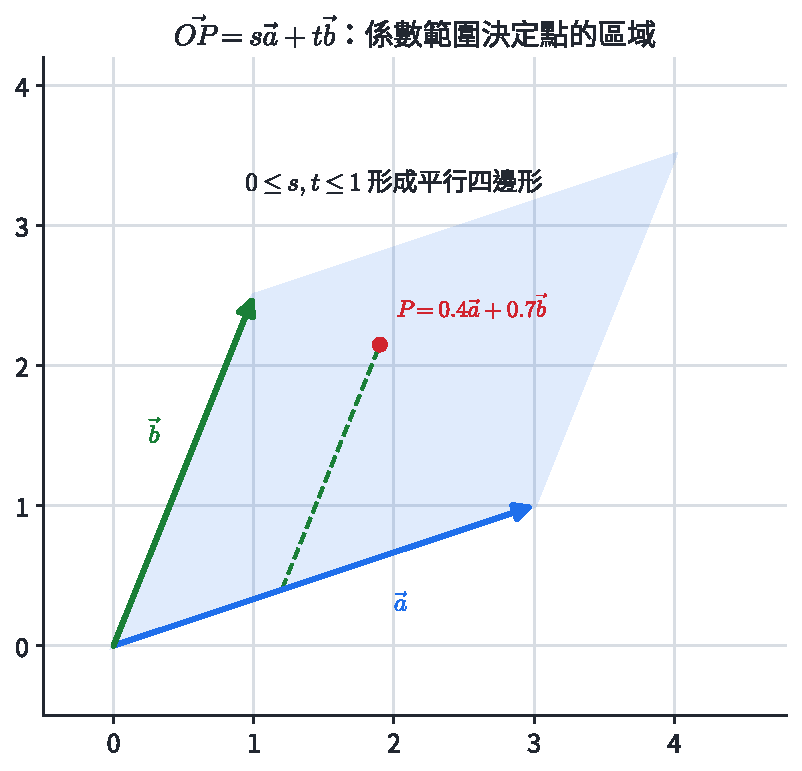
\includegraphics[width=0.86\linewidth,height=\textheight,keepaspectratio,alt={線性組合係數形成的區域}]{assets/數B3-3-線性組合區域.pdf}
\caption{線性組合係數形成的區域}
\end{figure}

圖中 \(\overrightarrow{OP}=s\vec a+t\vec b\) 且 \(0\le s,t\le1\)。\(s\vec a\) 在線段 \(O\) 到 \(A\) 上移動，從該點再加 \(t\vec b\)，便掃過整個平行四邊形。

\subsection{示範 1｜解線性組合係數}\label{ux793aux7bc4-1ux89e3ux7ddaux6027ux7d44ux5408ux4fc2ux6578}

已知 \(\vec a=(2,1)\)、\(\vec b=(-1,3)\)，把 \(\vec p=(7,1)\) 寫成 \(x\vec a+y\vec b\)。

\textbf{解。}

\[
(7,1)=(2x-y,x+3y),
\]

所以 \(2x-y=7\)、\(x+3y=1\)。解得

\[
x=\frac{22}{7},\qquad y=-\frac57.
\]

\subsection{示範 2｜由係數範圍求區域頂點}\label{ux793aux7bc4-2ux7531ux4fc2ux6578ux7bc4ux570dux6c42ux5340ux57dfux9802ux9ede}

設 \(\vec a=(3,0)\)、\(\vec b=(1,2)\)，\(\overrightarrow{OP}=s\vec a+t\vec b\)，其中 \(-1\le s\le1\)、\(0\le t\le2\)。求區域的四個頂點。

\textbf{解。} 係數矩形的四個角映成

\[
-\vec a=(-3,0),\quad \vec a=(3,0),
\]

\[
-\vec a+2\vec b=(-1,4),\quad \vec a+2\vec b=(5,4).
\]

四點依次連成平行四邊形。

\subsection{3.2 分節練習}\label{ux5206ux7bc0ux7df4ux7fd2-2}

\begin{enumerate}
\def\labelenumi{\arabic{enumi}.}
\tightlist
\item
  \(\vec a=(1,2)\)、\(\vec b=(3,-1)\)，將 \((11,1)\) 寫成 \(x\vec a+y\vec b\)。
\item
  判斷 \((2,4)\)、\((-1,-2)\) 能否作為平面的兩個基準方向。
\item
  \(\overrightarrow{OP}=s(2,0)+t(0,3)\)，\(0\le s,t\le1\)，求區域面積。
\item
  伸縮機構的端點位移為 \(4\vec a+4\vec b\)。若 \(\vec a=(3,-4)\)、\(\vec b=(1,2)\)，求端點位移與長度。
\end{enumerate}

\subsection{3.3 分節練習解析}\label{ux5206ux7bc0ux7df4ux7fd2ux89e3ux6790-2}

\begin{enumerate}
\def\labelenumi{\arabic{enumi}.}
\tightlist
\item
  \((x+3y,2x-y)=(11,1)\)，解得 \((x,y)=(2,3)\)。
\item
  \((2,4)=-2(-1,-2)\)，兩向量平行，無法唯一表示整個平面的向量。
\item
  兩邊長為 \(2\)、\(3\) 且垂直，面積為 \(6\)。
\item
  位移 \(4(3,-4)+4(1,2)=(16,-8)\)；長度 \(8\sqrt5\)。
\end{enumerate}

\section{4. 內分點與外分點}\label{ux5167ux5206ux9edeux8207ux5916ux5206ux9ede}

\subsection{4.1 以比例定位直線上的點}\label{ux4ee5ux6bd4ux4f8bux5b9aux4f4dux76f4ux7ddaux4e0aux7684ux9ede}

若 \(P\) 在線段 \(AB\) 上，且 \(AP:PB=m:n\)，其中 \(m,n>0\)，則

\[
\overrightarrow{OP}
=\frac{n\overrightarrow{OA}+m\overrightarrow{OB}}{m+n}.
\]

因 \(\overrightarrow{AP}=\dfrac{m}{m+n}\overrightarrow{AB}\)，所以

\[
\overrightarrow{OP}=\overrightarrow{OA}+\frac{m}{m+n}(\overrightarrow{OB}-\overrightarrow{OA}),
\]

整理即得內分公式。

\begin{figure}
\centering
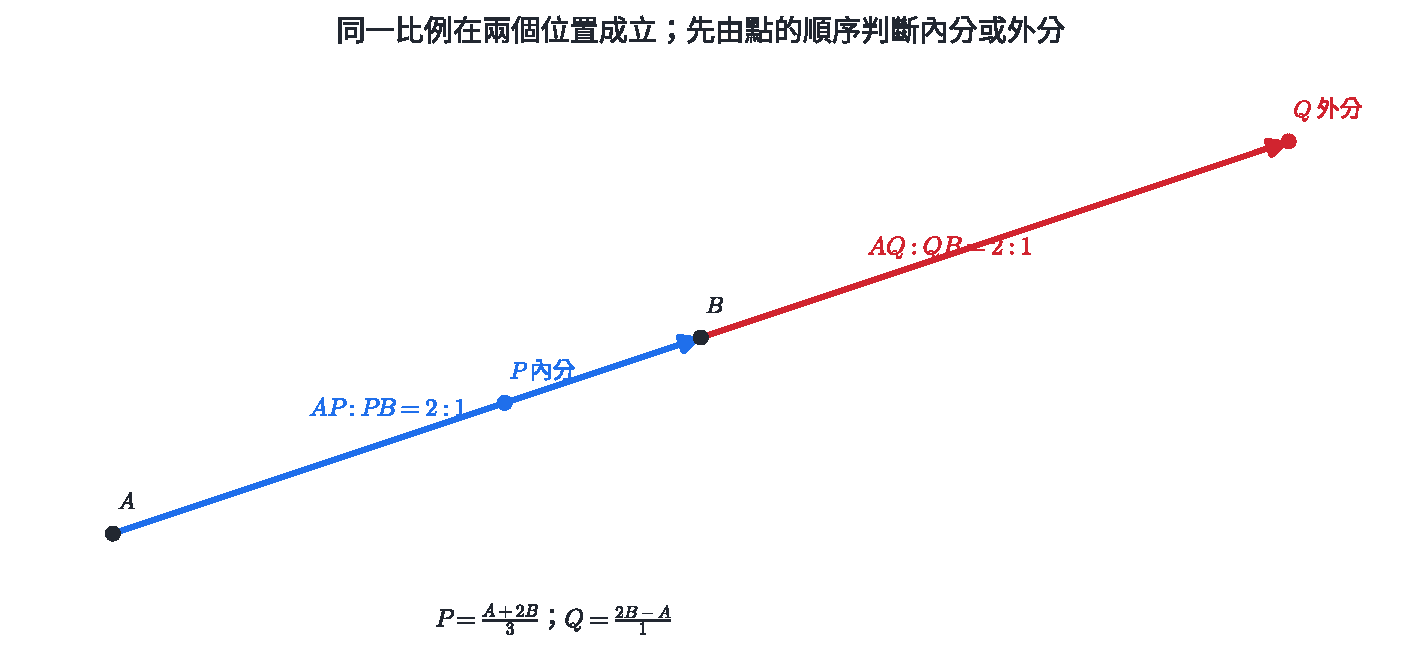
\includegraphics[width=0.94\linewidth,height=\textheight,keepaspectratio,alt={內分點與外分點的位置和方向}]{assets/數B3-3-內分與外分.pdf}
\caption{內分點與外分點的位置和方向}
\end{figure}

若 \(Q\) 在 \(B\) 的外側且 \(AQ:QB=m:n\)，其中 \(m>n>0\)，則

\[
\overrightarrow{OQ}
=\frac{m\overrightarrow{OB}-n\overrightarrow{OA}}{m-n}.
\]

圖中 \(AP:PB=2:1\) 的內分點在 \(A,B\) 之間；\(AQ:QB=2:1\) 的外分點在 \(B\) 外側。點的順序決定分母使用和或差。

\subsection{示範 1｜內分點坐標}\label{ux793aux7bc4-1ux5167ux5206ux9edeux5750ux6a19}

\(A(-2,5)\)、\(B(7,-1)\)，點 \(P\) 滿足 \(AP:PB=2:1\)。求 \(P\)。

\textbf{解。}

\[
P=\frac{A+2B}{3}
=\left(\frac{-2+14}{3},\frac{5-2}{3}\right)=(4,1).
\]

\(\overrightarrow{AP}=(6,-4)\) 是 \(\overrightarrow{PB}=(3,-2)\) 的 \(2\) 倍。

\subsection{示範 2｜同一比例的內、外兩解}\label{ux793aux7bc4-2ux540cux4e00ux6bd4ux4f8bux7684ux5167ux5916ux5169ux89e3}

\(A(0,0)\)、\(B(6,3)\)，求直線 \(AB\) 上所有滿足 \(AP:BP=3:2\) 的點。

\textbf{解。} 內分點與外分點分別為

\[
P_1=\frac{2A+3B}{5}=\left(\frac{18}{5},\frac95\right),
\]

\[
P_2=\frac{3B-2A}{3-2}=(18,9).
\]

兩點都滿足距離比 \(3:2\)，位置分別在 \(A,B\) 之間與 \(B\) 外側。

\subsection{4.2 分節練習}\label{ux5206ux7bc0ux7df4ux7fd2-3}

\begin{enumerate}
\def\labelenumi{\arabic{enumi}.}
\tightlist
\item
  \(A(1,4)\)、\(B(9,-2)\)，求 \(AP:PB=3:1\) 的內分點。
\item
  線段 \(AB\) 的中點為 \(M(2,-3)\)，已知 \(A(-4,5)\)，求 \(B\)。
\item
  \(A(2,1)\)、\(B(5,7)\)，求 \(AQ:QB=2:1\) 且 \(Q\) 在 \(B\) 外側的坐標。
\item
  感測器位於 \(A(-2,0)\)、\(B(8,0)\)。定位點到 \(A,B\) 的距離比為 \(3:2\)，且點在線段 \(AB\) 上，求坐標。
\end{enumerate}

\subsection{4.3 分節練習解析}\label{ux5206ux7bc0ux7df4ux7fd2ux89e3ux6790-3}

\begin{enumerate}
\def\labelenumi{\arabic{enumi}.}
\tightlist
\item
  \(P=(A+3B)/4=(7,-1/2)\)。
\item
  \(M=(A+B)/2\)，所以 \(B=2M-A=(8,-11)\)。
\item
  \(Q=(2B-A)/(2-1)=(8,13)\)；距離比為 \(2:1\)。
\item
  \(P=(2A+3B)/5=(4,0)\)。\(AP=6\)、\(PB=4\)，比例 \(3:2\)。
\end{enumerate}

\section{5. 縮放、平移與設計坐標}\label{ux7e2eux653eux5e73ux79fbux8207ux8a2dux8a08ux5750ux6a19}

\subsection{5.1 向量形式的圖形變換}\label{ux5411ux91cfux5f62ux5f0fux7684ux5716ux5f62ux8b8aux63db}

以原點為中心，倍率為 \(r\) 的縮放把點 \(P\) 送到 \(P'\)：

\[
\overrightarrow{OP'}=r\overrightarrow{OP}.
\]

所有長度乘 \(|r|\)，所有面積乘 \(r^2\)。再平移向量 \(\vec t=(a,b)\)，得到

\[
\overrightarrow{OP'}=r\overrightarrow{OP}+\vec t.
\]

\begin{figure}
\centering
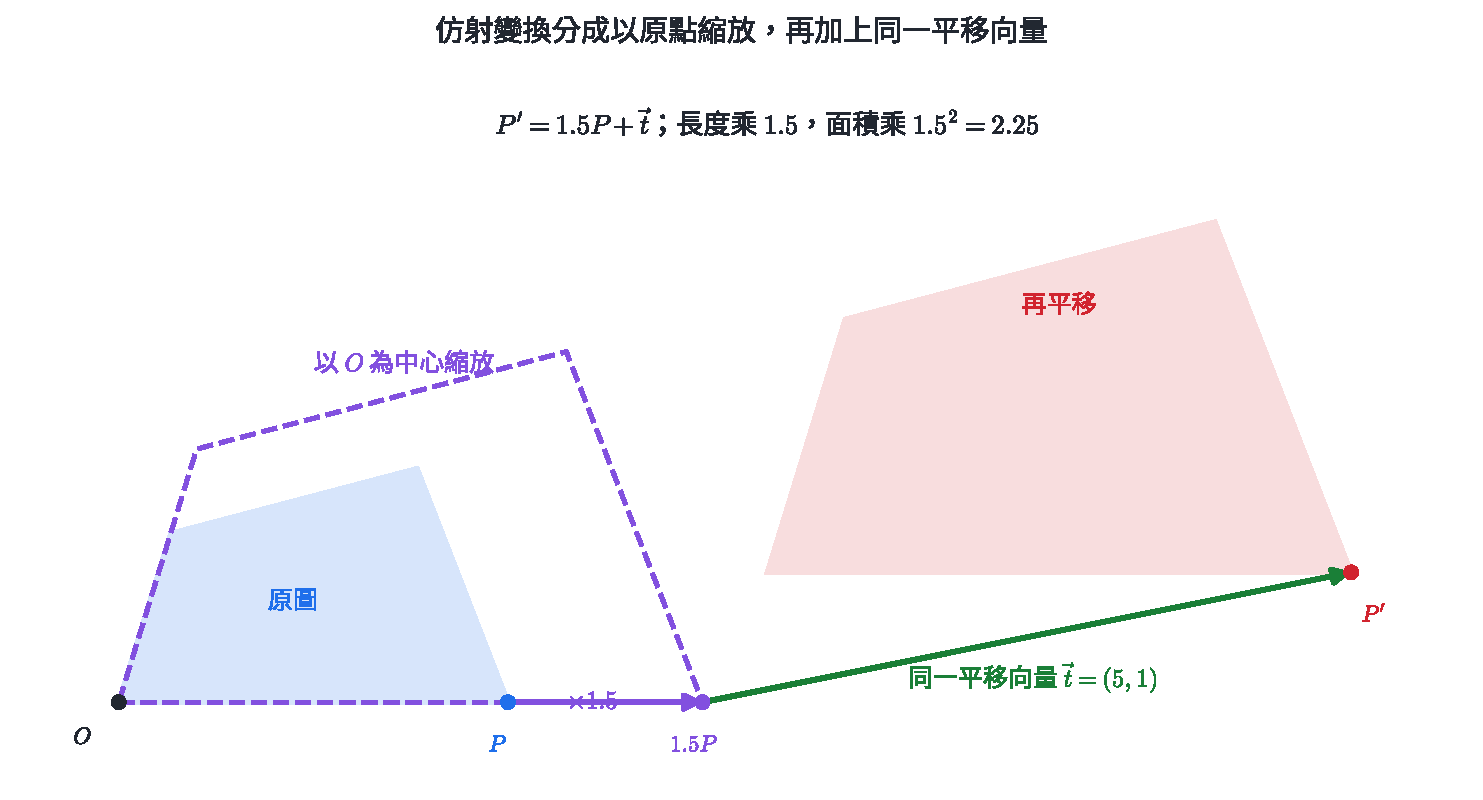
\includegraphics[width=0.9\linewidth,height=\textheight,keepaspectratio,alt={縮放與平移的長度面積倍率}]{assets/數B3-3-縮放與平移.pdf}
\caption{縮放與平移的長度面積倍率}
\end{figure}

相對位置差滿足 \(\overrightarrow{P'Q'}=r\overrightarrow{PQ}\)，因為平移量在兩位置向量相減時消去，縮放後的圖形保持相似。

\subsection{示範 1｜點的縮放和平移}\label{ux793aux7bc4-1ux9edeux7684ux7e2eux653eux548cux5e73ux79fb}

點 \(P(-2,3)\) 先以原點為中心放大 \(2\) 倍，再平移 \((5,-1)\)。求新坐標。

\textbf{解。}

\[
P'=2(-2,3)+(5,-1)=(1,5).
\]

\subsection{示範 2｜由面積倍率反求縮放倍率}\label{ux793aux7bc4-2ux7531ux9762ux7a4dux500dux7387ux53cdux6c42ux7e2eux653eux500dux7387}

一張圖等比例縮放後面積為原來的 \(0.64\) 倍，且圖形方向保持。求長度倍率。

\textbf{解。} 設長度倍率為 \(r>0\)：

\[
r^2=0.64\Rightarrow r=0.8.
\]

所有長度縮成原來的 \(80\%\)。

\subsection{5.2 分節練習}\label{ux5206ux7bc0ux7df4ux7fd2-4}

\begin{enumerate}
\def\labelenumi{\arabic{enumi}.}
\tightlist
\item
  點 \((4,-3)\) 經 \(P'=\frac12P+(-1,5)\) 後坐標為何？
\item
  三角形面積為 \(18\)，以倍率 \(-3\) 縮放後面積為何？
\item
  \(P',Q'\) 由 \(P,Q\) 經 \(X'=2X+(3,-4)\) 得到。若 \(\overrightarrow{PQ}=(-1,5)\)，求 \(\overrightarrow{P'Q'}\)。
\item
  圖像寬 \(1200\) 像素、高 \(800\) 像素，等比例縮小到面積為原來的 \(36\%\)。求新尺寸。
\end{enumerate}

\subsection{5.3 分節練習解析}\label{ux5206ux7bc0ux7df4ux7fd2ux89e3ux6790-4}

\begin{enumerate}
\def\labelenumi{\arabic{enumi}.}
\tightlist
\item
  \(P'=(2,-3/2)+(-1,5)=(1,7/2)\)。
\item
  面積倍率為 \((-3)^2=9\)，新面積 \(162\)。
\item
  \(\overrightarrow{P'Q'}=2\overrightarrow{PQ}=(-2,10)\)。
\item
  長度倍率為 \(\sqrt{0.36}=0.6\)，新尺寸為 \(720\times480\) 像素。
\end{enumerate}

\section{6. 向量夾角、內積與垂直判定}\label{ux5411ux91cfux593eux89d2ux5167ux7a4dux8207ux5782ux76f4ux5224ux5b9a}

\subsection{6.1 內積的幾何與坐標定義}\label{ux5167ux7a4dux7684ux5e7eux4f55ux8207ux5750ux6a19ux5b9aux7fa9}

把兩個非零向量平移到共同起點，夾角 \(\theta\) 取 \(0^\circ\le\theta\le180^\circ\)。\textbf{內積}定義為

\[
\vec a\cdot\vec b=|\vec a|\,|\vec b|\cos\theta.
\]

若 \(\vec a=(a_1,a_2)\)、\(\vec b=(b_1,b_2)\)，則

\[
\vec a\cdot\vec b=a_1b_1+a_2b_2.
\]

坐標公式可由餘弦定理推得。令 \(\vec a=\overrightarrow{OA}\)、\(\vec b=\overrightarrow{OB}\)，則 \(\overrightarrow{AB}=\vec b-\vec a\)。一方面

\[
|\vec b-\vec a|^2=|\vec a|^2+|\vec b|^2-2|\vec a||\vec b|\cos\theta,
\]

另一方面逐分量展開得到

\[
|\vec b-\vec a|^2=|\vec a|^2+|\vec b|^2-2(a_1b_1+a_2b_2).
\]

比較兩式即得坐標公式。

\begin{figure}
\centering
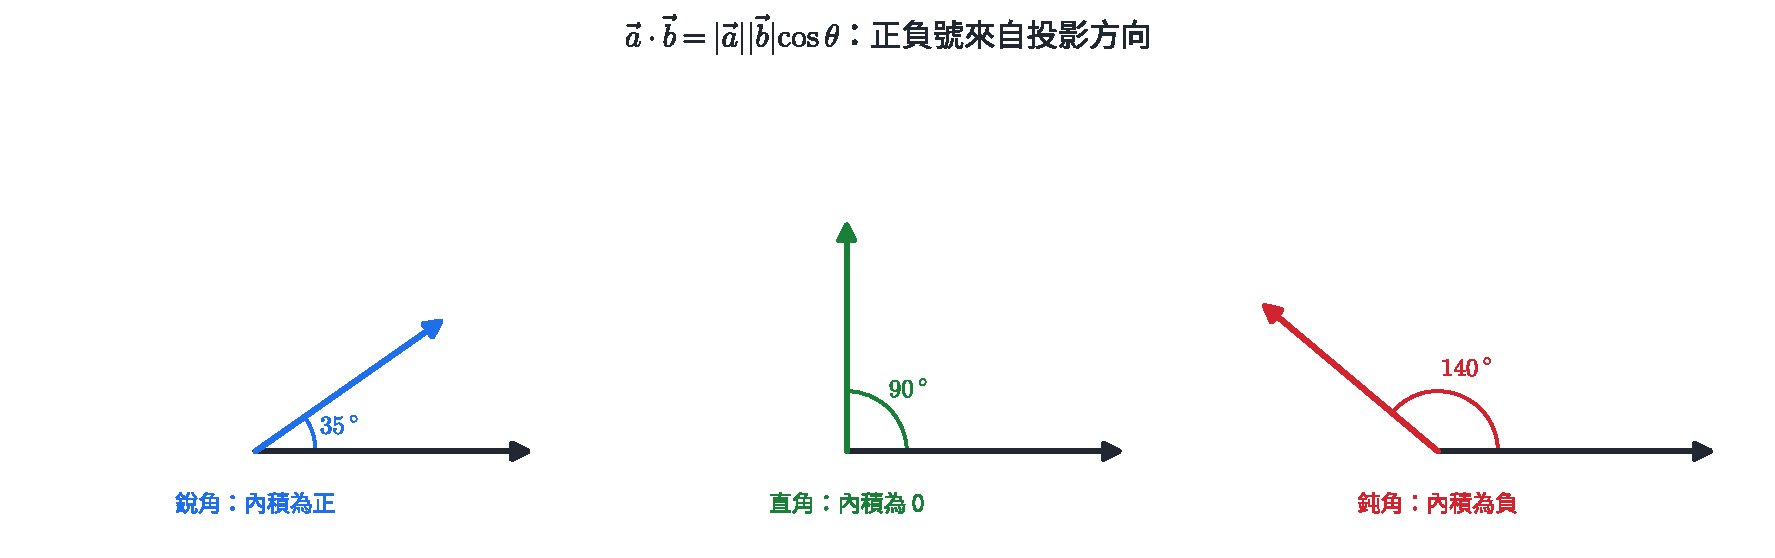
\includegraphics[width=0.96\linewidth,height=\textheight,keepaspectratio,alt={夾角與內積的正負}]{assets/數B3-3-夾角與內積.pdf}
\caption{夾角與內積的正負}
\end{figure}

圖中銳角、直角、鈍角分別使 \(\cos\theta\) 為正、零、負。因此對非零向量，

\[
\vec a\perp\vec b\quad\Longleftrightarrow\quad\vec a\cdot\vec b=0.
\]

力 \(\vec F\) 使物體產生位移 \(\vec s\) 時，定力所作的功為

\[
W=\vec F\cdot\vec s=|\vec F||\vec s|\cos\theta.
\]

功只計入力沿位移方向的分量，單位是焦耳（J）。

\subsection{示範 1｜由內積求夾角}\label{ux793aux7bc4-1ux7531ux5167ux7a4dux6c42ux593eux89d2}

\(\vec a=(3,4)\)、\(\vec b=(4,-3)\)，求夾角。

\textbf{解。}

\[
\vec a\cdot\vec b=3\cdot4+4(-3)=0.
\]

兩向量皆非零，因此夾角為 \(90^\circ\)。

\subsection{示範 2｜斜拉力所作的功}\label{ux793aux7bc4-2ux659cux62c9ux529bux6240ux4f5cux7684ux529f}

大小 \(80\text{ N}\) 的力與水平位移方向夾 \(60^\circ\)，物體移動 \(15\text{ m}\)。求功。

\textbf{解。}

\[
W=80\cdot15\cos60^\circ=600\text{ J}.
\]

沿位移方向的有效力為 \(80\cos60^\circ=40\text{ N}\)，再乘位移也得到 \(600\text{ J}\)。

\subsection{6.2 分節練習}\label{ux5206ux7bc0ux7df4ux7fd2-5}

\begin{enumerate}
\def\labelenumi{\arabic{enumi}.}
\tightlist
\item
  求 \((2,-5)\cdot(3,4)\)。
\item
  已知 \(|\vec a|=4\)、\(|\vec b|=6\)、夾角 \(120^\circ\)，求 \(\vec a\cdot\vec b\)。
\item
  求 \(k\)，使 \((k,2)\perp(3,-6)\)。
\item
  大小 \(50\text{ N}\) 的力與位移夾 \(30^\circ\)，位移 \(8\text{ m}\)。求功。
\item
  \(A(1,2)\)、\(B(5,4)\)、\(C(-1,6)\)，判斷 \(\angle BAC\) 的類型。
\end{enumerate}

\subsection{6.3 分節練習解析}\label{ux5206ux7bc0ux7df4ux7fd2ux89e3ux6790-5}

\begin{enumerate}
\def\labelenumi{\arabic{enumi}.}
\tightlist
\item
  \(2\cdot3+(-5)\cdot4=-14\)。
\item
  \(4\cdot6\cos120^\circ=-12\)。
\item
  \(3k+2(-6)=0\)，得 \(k=4\)。
\item
  \(W=50\cdot8\cos30^\circ=200\sqrt3\text{ J}\)。
\item
  \(\overrightarrow{AB}=(4,2)\)、\(\overrightarrow{AC}=(-2,4)\)，內積 \(-8+8=0\)，所以是直角。
\end{enumerate}

\section{7. 內積性質與向量長度}\label{ux5167ux7a4dux6027ux8ceaux8207ux5411ux91cfux9577ux5ea6}

\subsection{7.1 代數展開}\label{ux4ee3ux6578ux5c55ux958b}

內積滿足

\[
\vec a\cdot\vec b=\vec b\cdot\vec a,
\]

\[
(k\vec a)\cdot\vec b=k(\vec a\cdot\vec b),
\]

\[
(\vec a+\vec b)\cdot\vec c
=\vec a\cdot\vec c+\vec b\cdot\vec c,
\]

\[
\vec a\cdot\vec a=|\vec a|^2.
\]

因此向量和與差的長度可展開為

\[
|\vec a+\vec b|^2=|\vec a|^2+2\vec a\cdot\vec b+|\vec b|^2,
\]

\[
|\vec a-\vec b|^2=|\vec a|^2-2\vec a\cdot\vec b+|\vec b|^2.
\]

\begin{figure}
\centering
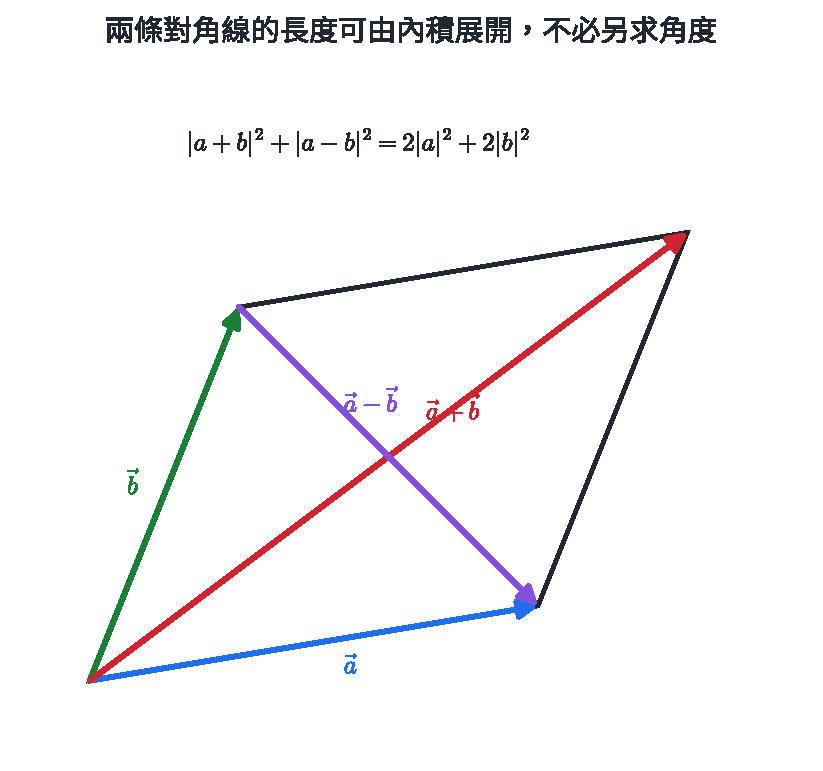
\includegraphics[width=0.86\linewidth,height=\textheight,keepaspectratio,alt={內積展開與平行四邊形對角線}]{assets/數B3-3-內積展開與對角線.pdf}
\caption{內積展開與平行四邊形對角線}
\end{figure}

兩式相加得到平行四邊形法則：

\[
|\vec a+\vec b|^2+|\vec a-\vec b|^2
=2|\vec a|^2+2|\vec b|^2.
\]

它把兩條對角線長度與四邊長連在一起。

\subsection{示範 1｜求向量組合的長度}\label{ux793aux7bc4-1ux6c42ux5411ux91cfux7d44ux5408ux7684ux9577ux5ea6}

已知 \(|\vec a|=3\)、\(|\vec b|=4\)、夾角 \(60^\circ\)，求 \(|2\vec a-\vec b|\)。

\textbf{解。} 先算 \(\vec a\cdot\vec b=3\cdot4\cos60^\circ=6\)。

\[
|2\vec a-\vec b|^2
=4|\vec a|^2-4\vec a\cdot\vec b+|\vec b|^2
=36-24+16=28.
\]

所以 \(|2\vec a-\vec b|=2\sqrt7\)。

\subsection{示範 2｜由兩條對角線反求邊長關係}\label{ux793aux7bc4-2ux7531ux5169ux689dux5c0dux89d2ux7ddaux53cdux6c42ux908aux9577ux95dcux4fc2}

平行四邊形兩邊向量為 \(\vec a,\vec b\)，已知 \(|\vec a+\vec b|=10\)、\(|\vec a-\vec b|=6\)、\(|\vec a|=5\)。求 \(|\vec b|\)。

\textbf{解。} 套用平行四邊形法則：

\[
10^2+6^2=2\cdot5^2+2|\vec b|^2.
\]

\[
136=50+2|\vec b|^2\Rightarrow |\vec b|^2=43.
\]

所以 \(|\vec b|=\sqrt{43}\)。

\subsection{7.2 分節練習}\label{ux5206ux7bc0ux7df4ux7fd2-6}

\begin{enumerate}
\def\labelenumi{\arabic{enumi}.}
\tightlist
\item
  已知 \(|\vec a|=2\)、\(|\vec b|=5\)、\(\vec a\cdot\vec b=-3\)，求 \(|\vec a+\vec b|\)。
\item
  已知 \(|\vec a+\vec b|=7\)、\(|\vec a|=3\)、\(|\vec b|=4\)，求 \(\vec a\cdot\vec b\)。
\item
  證明：若 \(|\vec a+\vec b|=|\vec a-\vec b|\)，則 \(\vec a\perp\vec b\)。
\item
  菱形邊長為 \(5\)，其中一條對角線長為 \(6\)，求另一條對角線長。
\item
  已知 \(|\vec u|=|\vec v|=2\)，且 \(\vec u+\vec v\) 與 \(\vec u\) 的夾角為 \(30^\circ\)，求 \(\vec u\cdot\vec v\)。
\end{enumerate}

\subsection{7.3 分節練習解析}\label{ux5206ux7bc0ux7df4ux7fd2ux89e3ux6790-6}

\begin{enumerate}
\def\labelenumi{\arabic{enumi}.}
\tightlist
\item
  \(|\vec a+\vec b|^2=4+2(-3)+25=23\)，故長度為 \(\sqrt{23}\)。
\item
  \(49=9+16+2\vec a\cdot\vec b\)，故內積為 \(12\)。
\item
  兩邊平方後相減，得到 \(4\vec a\cdot\vec b=0\)。兩向量非零時即互相垂直。
\item
  設另一對角線長 \(d\)。平行四邊形法則給 \(6^2+d^2=4(5^2)\)，所以 \(d=8\)。
\item
  等長向量構成菱形，\(\vec u+\vec v\) 平分夾角，故 \(\vec u,\vec v\) 夾角為 \(60^\circ\)；內積 \(2\cdot2\cos60^\circ=2\)。
\end{enumerate}

\section{8. 正射影、向量分解與距離}\label{ux6b63ux5c04ux5f71ux5411ux91cfux5206ux89e3ux8207ux8dddux96e2}

\subsection{8.1 正射影公式}\label{ux6b63ux5c04ux5f71ux516cux5f0f}

給定向量 \(\vec a\) 與非零向量 \(\vec b\)，\(\vec a\) 在 \(\vec b\) 上的\textbf{正射影向量}為

\[
\operatorname{proj}_{\vec b}\vec a
=\frac{\vec a\cdot\vec b}{|\vec b|^2}\vec b.
\]

推導時先設投影向量為 \(\vec v=t\vec b\)。垂直剩餘分量 \(\vec u=\vec a-\vec v\) 滿足 \(\vec u\cdot\vec b=0\)，所以

\[
(\vec a-t\vec b)\cdot\vec b=0
\Rightarrow t=\frac{\vec a\cdot\vec b}{|\vec b|^2}.
\]

\begin{figure}
\centering
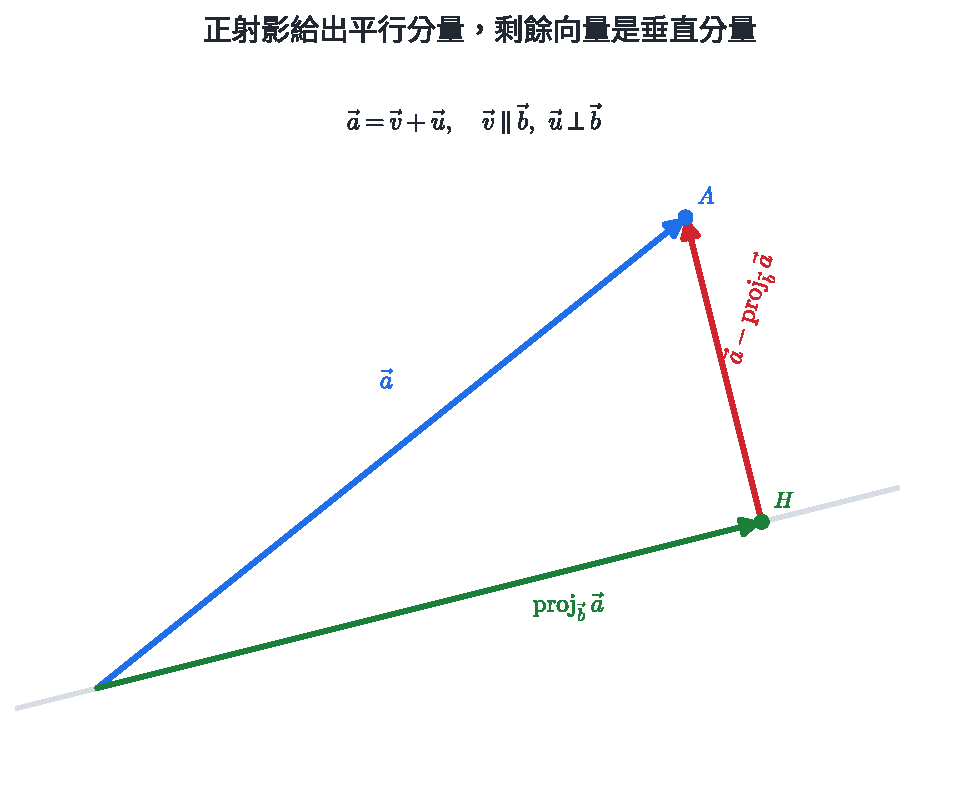
\includegraphics[width=0.88\linewidth,height=\textheight,keepaspectratio,alt={正射影與平行垂直分解}]{assets/數B3-3-正射影與分解.pdf}
\caption{正射影與平行垂直分解}
\end{figure}

圖中綠色向量是沿 \(\vec b\) 的平行分量，紅色向量是垂直分量：

\[
\vec a=\vec v+\vec u,\qquad \vec v\parallel\vec b,\qquad \vec u\perp\vec b.
\]

若直線 \(L\) 通過 \(A\)，方向向量為 \(\vec d\)，點 \(P\) 到 \(L\) 的投影點為

\[
H=A+\operatorname{proj}_{\vec d}\overrightarrow{AP}.
\]

點到直線距離為 \(PH\)。

\begin{figure}
\centering
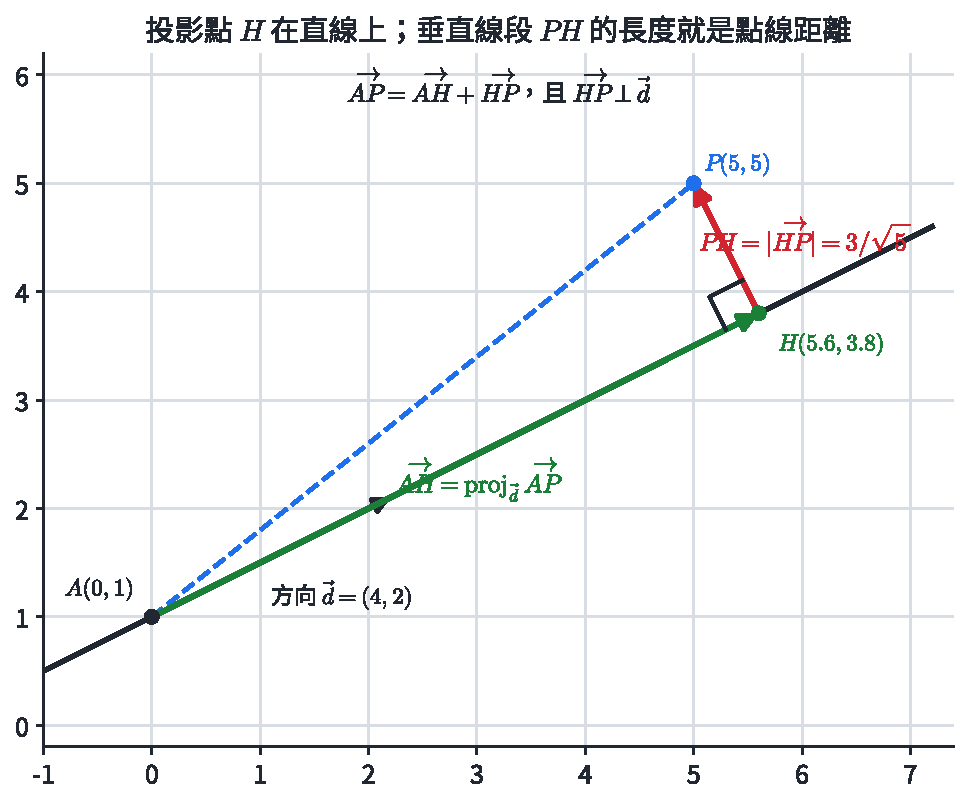
\includegraphics[width=0.88\linewidth,height=\textheight,keepaspectratio,alt={投影點與點到直線距離}]{assets/數B3-3-投影點與點線距離.pdf}
\caption{投影點與點到直線距離}
\end{figure}

\subsection{示範 1｜分解成平行與垂直分量}\label{ux793aux7bc4-1ux5206ux89e3ux6210ux5e73ux884cux8207ux5782ux76f4ux5206ux91cf}

把 \(\vec a=(6,5)\) 分解成平行於 \(\vec b=(2,1)\) 與垂直於 \(\vec b\) 的兩分量。

\textbf{解。}

\[
\vec v=\frac{(6,5)\cdot(2,1)}{2^2+1^2}(2,1)
=\frac{17}{5}(2,1)=\left(\frac{34}{5},\frac{17}{5}\right).
\]

\[
\vec u=\vec a-\vec v
=\left(-\frac45,\frac85\right).
\]

檢查 \(\vec u\cdot\vec b=-8/5+8/5=0\)。

\subsection{示範 2｜求投影點與點線距離}\label{ux793aux7bc4-2ux6c42ux6295ux5f71ux9edeux8207ux9edeux7ddaux8dddux96e2}

直線 \(L\) 通過 \(A(1,0)\)，方向向量為 \((2,1)\)。求 \(P(4,5)\) 在 \(L\) 上的投影點與距離。

\textbf{解。} \(\overrightarrow{AP}=(3,5)\)：

\[
\operatorname{proj}_{(2,1)}(3,5)
=\frac{11}{5}(2,1)=\left(\frac{22}{5},\frac{11}{5}\right).
\]

\[
H=A+\operatorname{proj}_{(2,1)}\overrightarrow{AP}
=\left(\frac{27}{5},\frac{11}{5}\right).
\]

\[
\overrightarrow{HP}=\left(-\frac75,\frac{14}{5}\right),\qquad
PH=\frac{7\sqrt5}{5}.
\]

\subsection{8.2 分節練習}\label{ux5206ux7bc0ux7df4ux7fd2-7}

\begin{enumerate}
\def\labelenumi{\arabic{enumi}.}
\tightlist
\item
  求 \((5,1)\) 在 \((1,2)\) 上的正射影向量。
\item
  把 \((4,-1)\) 分解成平行於 \((3,4)\) 與垂直於 \((3,4)\) 的分量。
\item
  直線通過原點且方向為 \((1,1)\)，求 \(P(4,0)\) 的投影點與距離。
\item
  棍子端點為 \(A(0,6)\)、\(B(8,0)\)，彈珠位於 \(P(5,8)\)，沿垂直棍子的方向落到 \(H\)。求 \(H\)。
\item
  一個大小 \(20\text{ N}\) 的力作用方向為 \((3,4)\)，求它在向東方向的有向分量大小。
\end{enumerate}

\subsection{8.3 分節練習解析}\label{ux5206ux7bc0ux7df4ux7fd2ux89e3ux6790-7}

\begin{enumerate}
\def\labelenumi{\arabic{enumi}.}
\tightlist
\item
  係數為 \((5+2)/5=7/5\)，投影為 \((7/5,14/5)\)。
\item
  投影係數為 \((12-4)/25=8/25\)，平行分量 \((24/25,32/25)\)；垂直分量 \((76/25,-57/25)\)。
\item
  投影為 \(((4,0)\cdot(1,1)/2)(1,1)=(2,2)\)；距離 \(|(2,-2)|=2\sqrt2\)。
\item
  \(\overrightarrow{AB}=(8,-6)\)、\(\overrightarrow{AP}=(5,2)\)。投影係數 \((40-12)/100=7/25\)，故 \(H=A+(56/25,-42/25)=(56/25,108/25)\)。
\item
  東向單位向量為 \((1,0)\)。力向量是 \(20(3/5,4/5)=(12,16)\)，東向有向分量為 \(12\text{ N}\)。
\end{enumerate}

\section{9. 直線法向量、直線方程式與夾角}\label{ux76f4ux7ddaux6cd5ux5411ux91cfux76f4ux7ddaux65b9ux7a0bux5f0fux8207ux593eux89d2}

\subsection{9.1 法向量}\label{ux6cd5ux5411ux91cf}

與直線垂直的非零向量稱為直線的\textbf{法向量}。直線

\[
ax+by+c=0
\]

的一個法向量是 \(\vec n=(a,b)\)。若直線通過 \(P(x_0,y_0)\)，以法向量 \((a,b)\) 表示，可寫成

\[
a(x-x_0)+b(y-y_0)=0.
\]

\begin{figure}
\centering
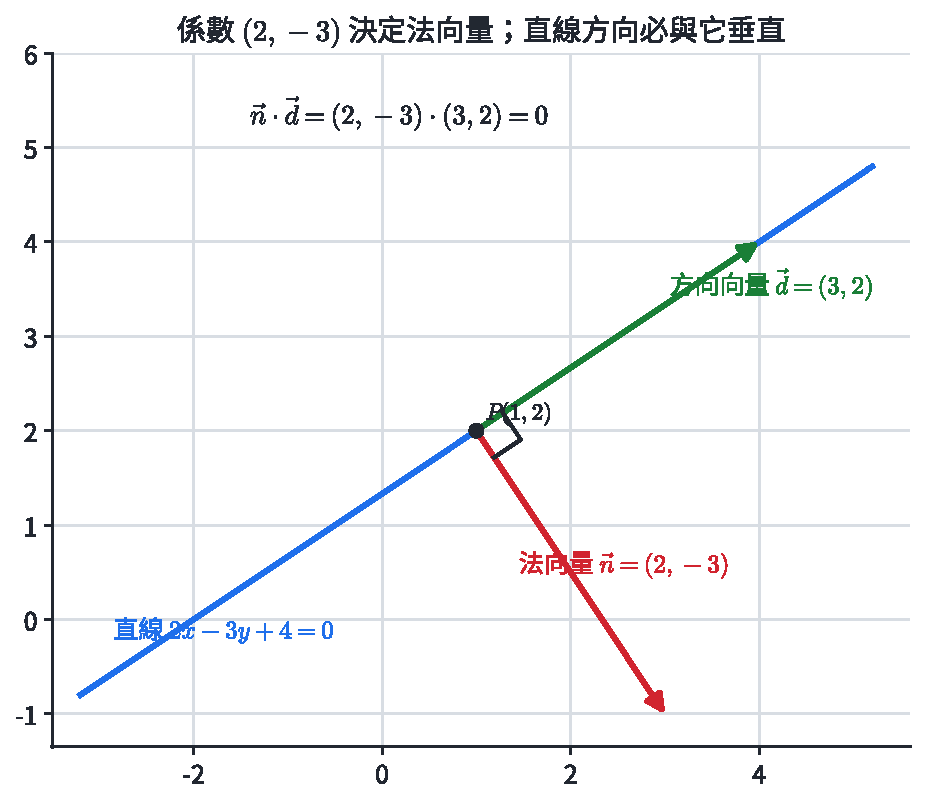
\includegraphics[width=0.86\linewidth,height=\textheight,keepaspectratio,alt={法向量與直線方向}]{assets/數B3-3-法向量與直線.pdf}
\caption{法向量與直線方向}
\end{figure}

圖中的法向量 \((2,-3)\) 與方向向量 \((3,2)\) 內積為 \(0\)。對直線上任一點 \(X\)，\(\overrightarrow{PX}\) 都與法向量垂直，因此 \(\vec n\cdot\overrightarrow{PX}=0\)，展開即為直線方程式。

兩直線的法向量分別為 \(\vec n_1,\vec n_2\) 時，可先求法向量夾角 \(\theta\)：

\[
\cos\theta=\frac{\vec n_1\cdot\vec n_2}{|\vec n_1||\vec n_2|}.
\]

兩直線形成的兩種角為 \(\theta\) 與 \(180^\circ-\theta\)；題目若問銳夾角，可取 \(|\cos\theta|\)。

\subsection{示範 1｜由法向量與一點寫直線}\label{ux793aux7bc4-1ux7531ux6cd5ux5411ux91cfux8207ux4e00ux9edeux5bebux76f4ux7dda}

求通過 \((2,-1)\)、法向量為 \((3,4)\) 的直線方程式。

\textbf{解。}

\[
3(x-2)+4(y+1)=0
\Rightarrow3x+4y-2=0.
\]

\subsection{示範 2｜求兩直線的銳夾角}\label{ux793aux7bc4-2ux6c42ux5169ux76f4ux7ddaux7684ux92b3ux593eux89d2}

\(L_1:2x-y+3=0\)，\(L_2:x+2y-4=0\)。求夾角。

\textbf{解。} 法向量為 \(\vec n_1=(2,-1)\)、\(\vec n_2=(1,2)\)：

\[
\vec n_1\cdot\vec n_2=2-2=0.
\]

兩法向量垂直，兩直線也垂直，夾角為 \(90^\circ\)。

\subsection{9.2 分節練習}\label{ux5206ux7bc0ux7df4ux7fd2-8}

\begin{enumerate}
\def\labelenumi{\arabic{enumi}.}
\tightlist
\item
  寫出直線 \(5x-2y+7=0\) 的一個法向量與一個方向向量。
\item
  求通過 \((-1,3)\)、法向量 \((4,-3)\) 的直線方程式。
\item
  判斷 \(3x+4y=1\) 與 \(4x-3y=8\) 的關係。
\item
  求 \(x+y=0\) 與 \(\sqrt3x-y+2=0\) 的銳夾角。
\item
  道路中心線方向為 \((4,3)\)，設計一條通過 \((6,2)\) 且與道路垂直的標線，求方程式。
\end{enumerate}

\subsection{9.3 分節練習解析}\label{ux5206ux7bc0ux7df4ux7fd2ux89e3ux6790-8}

\begin{enumerate}
\def\labelenumi{\arabic{enumi}.}
\tightlist
\item
  法向量可取 \((5,-2)\)；方向向量可取 \((2,5)\)，兩者內積為 \(0\)。
\item
  \(4(x+1)-3(y-3)=0\)，即 \(4x-3y+13=0\)。
\item
  法向量 \((3,4)\) 與 \((4,-3)\) 內積為 \(0\)，所以兩直線垂直。
\item
  法向量 \((1,1)\)、\((\sqrt3,-1)\) 的內積為 \(\sqrt3-1\)，長度皆為 \(\sqrt2\)、\(2\)。銳角餘弦為 \((\sqrt3-1)/(2\sqrt2)=\cos75^\circ\)，故夾角 \(75^\circ\)。
\item
  標線方向與道路垂直，所以道路方向 \((4,3)\) 可作標線法向量：\(4(x-6)+3(y-2)=0\)，即 \(4x+3y-30=0\)。
\end{enumerate}

\section{10. 單點透視與相似比例}\label{ux55aeux9edeux900fux8996ux8207ux76f8ux4f3cux6bd4ux4f8b}

\subsection{10.1 消失點、地平線與等分}\label{ux6d88ux5931ux9edeux5730ux5e73ux7ddaux8207ux7b49ux5206}

單點透視把一組與畫面垂直的空間平行線畫成通向同一點的直線；該點稱為\textbf{消失點}。與地面平行且通過觀察者眼睛高度的線稱為\textbf{地平線}，消失點位於地平線上。

\begin{figure}
\centering
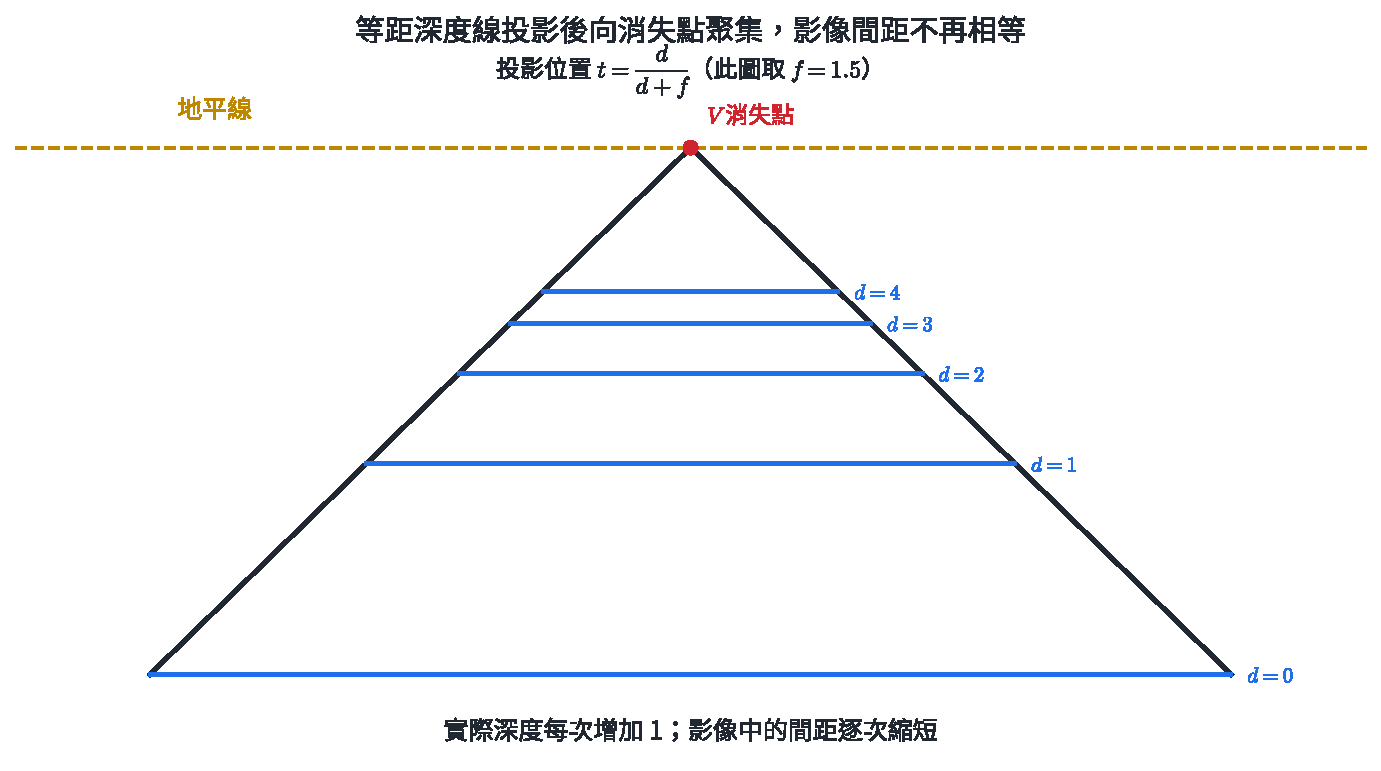
\includegraphics[width=0.92\linewidth,height=\textheight,keepaspectratio,alt={單點透視的消失點與深度線}]{assets/數B3-3-單點透視等分.pdf}
\caption{單點透視的消失點與深度線}
\end{figure}

圖中左右兩條深度線在 \(V\) 相交，橫向線保持互相平行。越接近 \(V\) 的橫線越短，對應物體距離觀察者越遠。等距深度在畫面上的間距會逐漸縮小，因此透視等分要用交叉線與相似三角形建構。

若眼睛 \(E\)、畫面與物體的對應點共線，投影前後的三角形相似。設畫面距眼睛 \(d\)，物體距眼睛 \(D\)，實際高度 \(H\)、畫面高度 \(h\)，則

\[
\frac{h}{H}=\frac{d}{D}.
\]

\begin{figure}
\centering
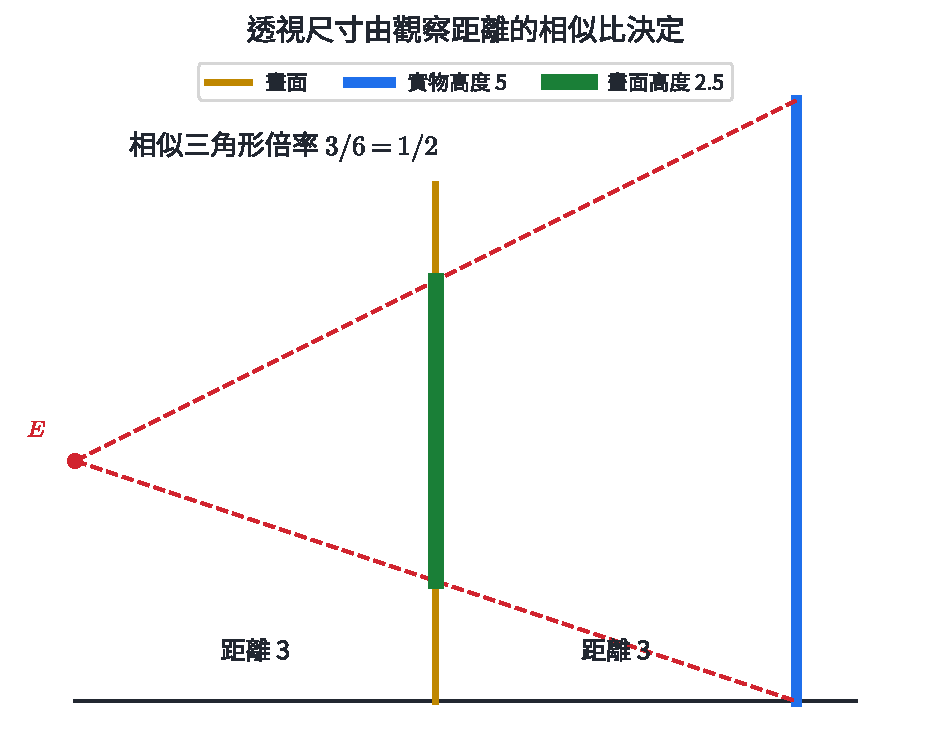
\includegraphics[width=0.9\linewidth,height=\textheight,keepaspectratio,alt={透視尺寸的相似三角形}]{assets/數B3-3-透視比例.pdf}
\caption{透視尺寸的相似三角形}
\end{figure}

圖中畫面距離是物體距離的一半，所以高度 \(5\) 在畫面上成為 \(2.5\)。同一深度平面上的所有長度都乘同一倍率。

\subsection{示範 1｜由距離求畫面高度}\label{ux793aux7bc4-1ux7531ux8dddux96e2ux6c42ux756bux9762ux9ad8ux5ea6}

畫面距眼睛 \(2\text{ m}\)，一根高 \(3\text{ m}\) 的柱子距眼睛 \(8\text{ m}\)。柱子在畫面上的高度是多少？

\textbf{解。}

\[
\frac{h}{3}=\frac{2}{8}\Rightarrow h=0.75\text{ m}.
\]

倍率 \(1/4\) 同時作用於柱子的寬與高。

\subsection{示範 2｜由兩個透視截面反求長度}\label{ux793aux7bc4-2ux7531ux5169ux500bux900fux8996ux622aux9762ux53cdux6c42ux9577ux5ea6}

同一組深度線通向消失點 \(V\)。兩個平行截面到 \(V\) 的距離分別為 \(6\) 與 \(10\)，較近 \(V\) 的截面寬為 \(9\)。求另一截面寬。

\textbf{解。} 截面寬與到消失點的對應距離成同比例：

\[
\frac{9}{w}=\frac{6}{10}
\Rightarrow w=15.
\]

另一截面離 \(V\) 較遠，所以圖上寬度較大，與 \(15>9\) 一致。

\subsection{10.2 分節練習}\label{ux5206ux7bc0ux7df4ux7fd2-9}

\begin{enumerate}
\def\labelenumi{\arabic{enumi}.}
\tightlist
\item
  透視圖中三條深度方向的線交於同一點 \(V\)。說明 \(V\) 的名稱與所在的水平參考線。
\item
  畫面距眼睛 \(1.5\text{ m}\)，物體距眼睛 \(6\text{ m}\)，物體高 \(2.4\text{ m}\)。求畫面高度。
\item
  兩個平行截面到消失點的距離比為 \(3:5\)，較近截面寬 \(12\)。求較遠截面寬。
\item
  透明屏風距眼睛 \(2\text{ m}\)，箱子距眼睛 \(5\text{ m}\)；箱頂比眼睛高 \(0.6\text{ m}\)。求箱頂投影相對眼睛高度。
\item
  走廊地磚的真實寬度相同。說明它們在透視圖中逐漸縮短的數學原因。
\end{enumerate}

\subsection{10.3 分節練習解析}\label{ux5206ux7bc0ux7df4ux7fd2ux89e3ux6790-9}

\begin{enumerate}
\def\labelenumi{\arabic{enumi}.}
\tightlist
\item
  \(V\) 是消失點，位於地平線上；地平線對應觀察者眼睛高度。
\item
  \(h/2.4=1.5/6\)，得 \(h=0.6\text{ m}\)。
\item
  \(12/w=3/5\)，得 \(w=20\)。
\item
  相對高度乘距離倍率 \(2/5\)，所以投影比眼睛高 \(0.6(2/5)=0.24\text{ m}\)。
\item
  每塊地磚的影像由相似三角形縮放；離眼睛越遠，\(d/D\) 越小，所以畫面長度越短，深度線同時趨向消失點。
\end{enumerate}

\section{11. A 系列紙張與自相似規格}\label{a-ux7cfbux5217ux7d19ux5f35ux8207ux81eaux76f8ux4f3cux898fux683c}

\subsection{11.1 長寬比與面積}\label{ux9577ux5becux6bd4ux8207ux9762ux7a4d}

設矩形長邊為 \(x\)、短邊為 \(y\)，沿長邊對半裁切後，小矩形旋轉 \(90^\circ\) 與原矩形相似。相似條件為

\[
\frac{x}{y}=\frac{y}{x/2}.
\]

因此

\[
x^2=2y^2,\qquad \frac{x}{y}=\sqrt2.
\]

\begin{figure}
\centering
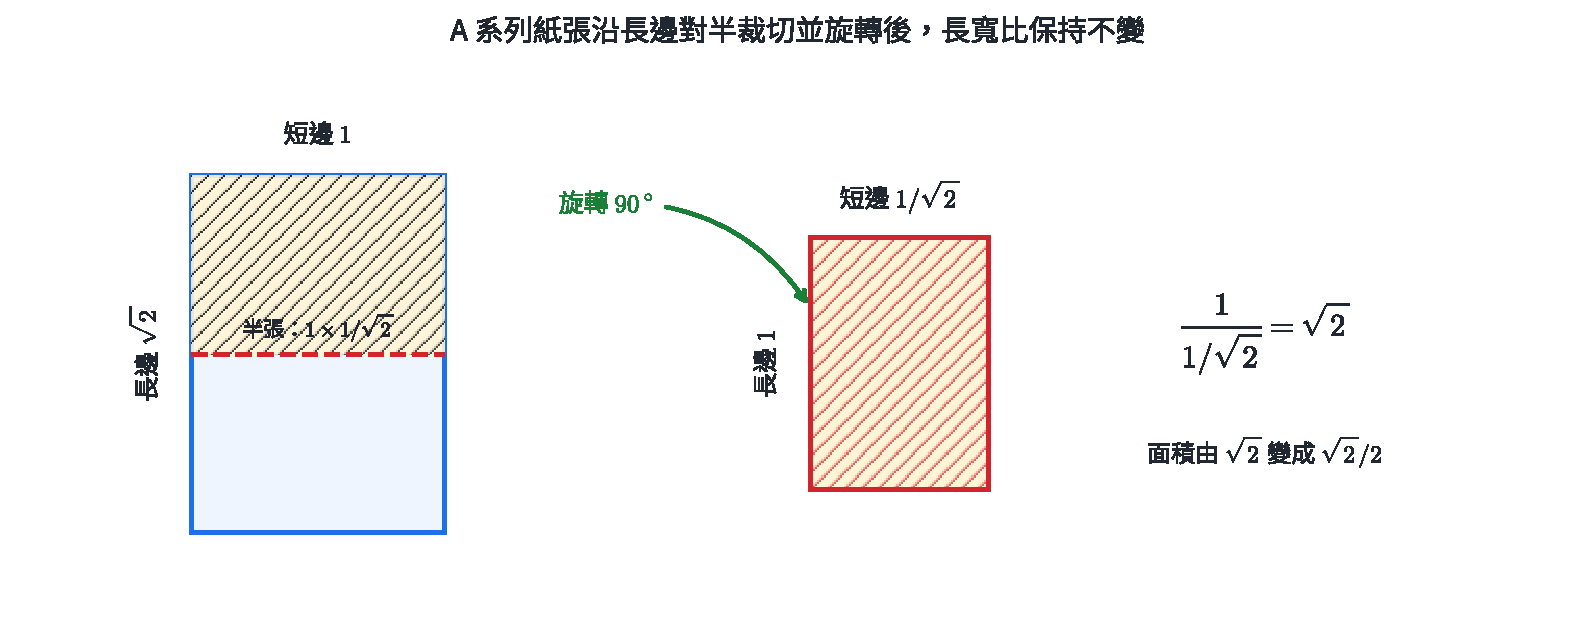
\includegraphics[width=0.9\linewidth,height=\textheight,keepaspectratio,alt={A系列紙張的自相似比例}]{assets/數B3-3-A系列紙張.pdf}
\caption{A系列紙張的自相似比例}
\end{figure}

A0 面積定為 \(1\text{ m}^2\)。每沿長邊對半裁切一次，面積減半：

\[
\text{A}n\text{ 面積}=2^{-n}\text{ m}^2.
\]

實際紙張尺寸以整數毫米表示，因此表列長寬會含四捨五入。理想模型的長寬比與面積關係用 \(\sqrt2\) 與 \(2^{-n}\) 計算。

\subsection{示範 1｜由 A0 面積求 A4 面積}\label{ux793aux7bc4-1ux7531-a0-ux9762ux7a4dux6c42-a4-ux9762ux7a4d}

求 A4 面積，分別用平方公尺與平方公分表示。

\textbf{解。} 從 A0 到 A4 裁切四次：

\[
A_4=2^{-4}=\frac1{16}\text{ m}^2.
\]

因 \(1\text{ m}^2=10000\text{ cm}^2\)，所以

\[
A_4=625\text{ cm}^2.
\]

\subsection{示範 2｜由一邊反求理想尺寸}\label{ux793aux7bc4-2ux7531ux4e00ux908aux53cdux6c42ux7406ux60f3ux5c3aux5bf8}

理想 A 系列紙張短邊為 \(210\text{ mm}\)，求長邊與面積。

\textbf{解。}

\[
x=210\sqrt2\approx296.98\text{ mm}.
\]

\[
A=210(210\sqrt2)=44100\sqrt2\approx62366\text{ mm}^2.
\]

規格表把長邊寫為 \(297\text{ mm}\)，是毫米整數化的結果。

\subsection{11.2 分節練習}\label{ux5206ux7bc0ux7df4ux7fd2-10}

\begin{enumerate}
\def\labelenumi{\arabic{enumi}.}
\tightlist
\item
  求理想 A3 的面積，單位為平方公尺。
\item
  A2 長邊為 \(594\text{ mm}\)，沿長邊對半裁切後所得 A3 的兩邊為何？
\item
  一張自相似紙的長邊為 \(40\text{ cm}\)，求短邊的理想值。
\item
  A0 面積為 \(1\text{ m}^2\)，求 A5 面積，單位為平方公分。
\item
  同一 A 系列中，A2 與 A5 的面積比為何？
\end{enumerate}

\subsection{11.3 分節練習解析}\label{ux5206ux7bc0ux7df4ux7fd2ux89e3ux6790-10}

\begin{enumerate}
\def\labelenumi{\arabic{enumi}.}
\tightlist
\item
  A3 面積為 \(2^{-3}=1/8\text{ m}^2\)。
\item
  A2 的短邊等於 A3 的長邊，即 \(420\text{ mm}\)；另一邊為 \(594/2=297\text{ mm}\)。
\item
  短邊 \(=40/\sqrt2=20\sqrt2\text{ cm}\)。
\item
  \(10000/2^5=312.5\text{ cm}^2\)。
\item
  相差三次裁切，所以 A2:A5 面積 \(=2^3:1=8:1\)。
\end{enumerate}

\section{12. 黃金分割、費氏數列與螺線}\label{ux9ec3ux91d1ux5206ux5272ux8cbbux6c0fux6578ux5217ux8207ux87baux7dda}

\subsection{12.1 黃金比例的方程}\label{ux9ec3ux91d1ux6bd4ux4f8bux7684ux65b9ux7a0b}

把線段分成長段 \(x\) 與短段 \(1\)，若

\[
\frac{x}{1}=\frac{x+1}{x},
\]

則稱為\textbf{黃金分割}。整理得到

\[
x^2-x-1=0.
\]

長度取正根：

\[
\varphi=\frac{1+\sqrt5}{2}\approx1.618034.
\]

因此 \(\varphi^2=\varphi+1\) 與 \(1/\varphi=\varphi-1\)。

費氏數列定義為

\[
F_1=F_2=1,\qquad F_{n+2}=F_{n+1}+F_n.
\]

它的前幾項為 \(1,1,2,3,5,8,13,\ldots\)。相鄰比 \(F_n/F_{n-1}\) 會在 \(\varphi\) 上下交替並逐漸接近它。

\begin{figure}
\centering
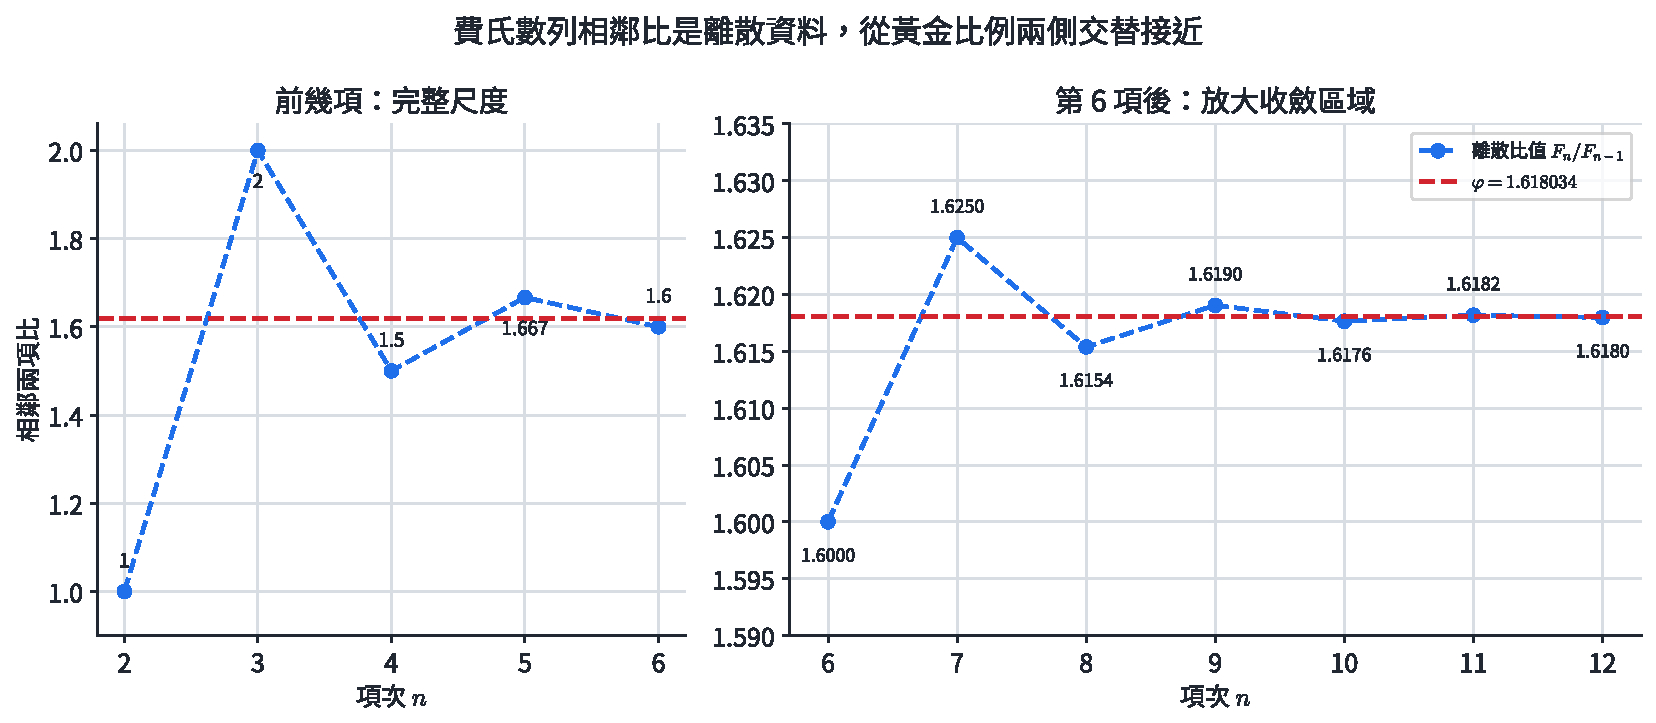
\includegraphics[width=0.88\linewidth,height=\textheight,keepaspectratio,alt={費氏數列相鄰比接近黃金比例}]{assets/數B3-3-費氏比值.pdf}
\caption{費氏數列相鄰比接近黃金比例}
\end{figure}

若把黃金矩形切去一個正方形，剩下的小矩形仍與原矩形相似。精確的黃金螺線每轉 \(90^\circ\)，半徑乘一次 \(\varphi\)。

\begin{figure}
\centering
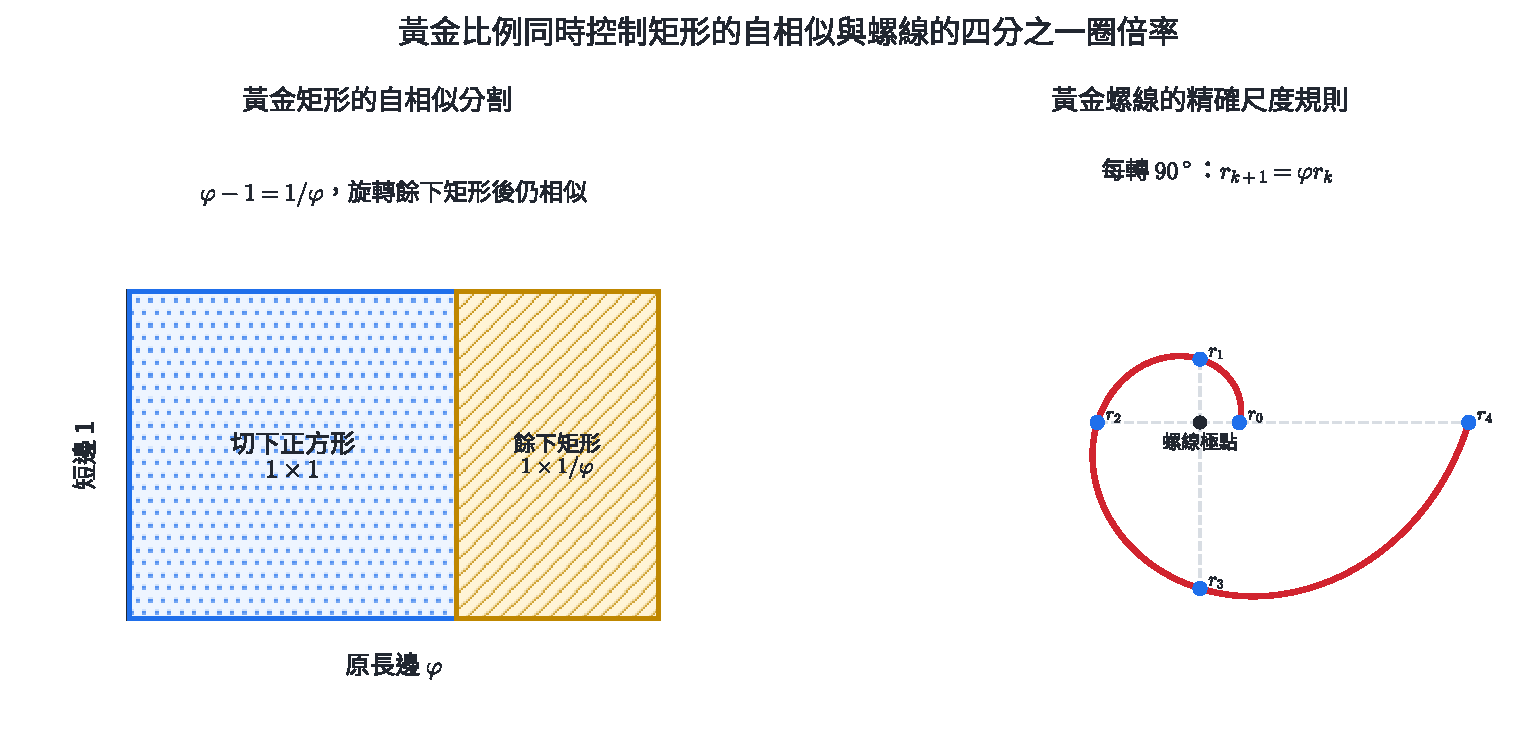
\includegraphics[width=0.88\linewidth,height=\textheight,keepaspectratio,alt={黃金矩形切除正方形後仍相似；黃金螺線每轉九十度半徑乘黃金比例}]{assets/數B3-3-黃金分割與方形螺線.pdf}
\caption{黃金矩形切除正方形後仍相似；黃金螺線每轉九十度半徑乘黃金比例}
\end{figure}

常見的方形螺線由連續正方形內的四分之一圓弧拼接，與精確的等角螺線屬於不同曲線。設計作品是否「美」也需要使用者、文化與功能資料支持；黃金比例在本節的可驗證內容是方程、自相似與數列比值。

\subsection{示範 1｜求黃金分割點}\label{ux793aux7bc4-1ux6c42ux9ec3ux91d1ux5206ux5272ux9ede}

線段 \(OA\) 長 \(10\)，點 \(B\) 在 \(OA\) 上，且長段 \(AB\)、短段 \(OB\) 構成黃金分割。求 \(OB\)。

\textbf{解。} 長段與短段比為 \(\varphi\)。若 \(OB=s\)，則 \(AB=10-s\) 且

\[
\frac{10-s}{s}=\varphi.
\]

因此

\[
s=\frac{10}{1+\varphi}=\frac{10}{\varphi^2}=5(3-\sqrt5).
\]

數值約為 \(3.820\)，而長段約為 \(6.180\)。

\subsection{示範 2｜計算費氏相鄰比}\label{ux793aux7bc4-2ux8a08ux7b97ux8cbbux6c0fux76f8ux9130ux6bd4}

從 \(F_1=F_2=1\) 算到 \(F_{10}\)，並比較 \(F_{10}/F_9\) 與 \(\varphi\)。

\textbf{解。} 依遞迴得到

\[
1,1,2,3,5,8,13,21,34,55.
\]

\[
\frac{F_{10}}{F_9}=\frac{55}{34}\approx1.617647.
\]

與 \(\varphi\approx1.618034\) 的差約 \(0.000387\)。

\subsection{12.2 分節練習}\label{ux5206ux7bc0ux7df4ux7fd2-11}

\begin{enumerate}
\def\labelenumi{\arabic{enumi}.}
\tightlist
\item
  解 \(x^2-x-1=0\)，並指出適合作為長度比的根。
\item
  已知黃金矩形短邊為 \(8\)，求長邊與切去正方形後餘下矩形的短邊。
\item
  寫出 \(F_{11}\) 與 \(F_{12}\)，並算 \(F_{12}/F_{11}\) 至小數第四位。
\item
  黃金長方形畫面寬 \(160\text{ cm}\)，求理想高度。
\item
  邊長依序為 \(1,2,3,5\) 的四個正方形內各畫四分之一圓，求弧長總和。
\end{enumerate}

\subsection{12.3 分節練習解析}\label{ux5206ux7bc0ux7df4ux7fd2ux89e3ux6790-11}

\begin{enumerate}
\def\labelenumi{\arabic{enumi}.}
\tightlist
\item
  根為 \((1\pm\sqrt5)/2\)；長度比取正根 \(\varphi\)。
\item
  長邊 \(8\varphi\)；切去 \(8\times8\) 正方形後，餘下矩形短邊 \(8\varphi-8=8(\varphi-1)=8/\varphi\)。
\item
  \(F_{11}=89\)、\(F_{12}=144\)；\(144/89\approx1.6180\)。
\item
  \(160/h=\varphi\)，所以 \(h=160/\varphi\approx98.9\text{ cm}\)。
\item
  每段弧長是 \((\pi/2)r\)，總和 \(=(\pi/2)(1+2+3+5)=11\pi/2\)。
\end{enumerate}

\section{13. 圓角、相似縮放與平面設計}\label{ux5713ux89d2ux76f8ux4f3cux7e2eux653eux8207ux5e73ux9762ux8a2dux8a08}

\subsection{13.1 圓弧與切線條件}\label{ux5713ux5f27ux8207ux5207ux7ddaux689dux4ef6}

圓與直線相切時，連接圓心與切點的半徑垂直於切線。若一個圓同時與角的兩邊相切，圓心到兩邊距離相等，所以圓心位於角平分線上。

\begin{figure}
\centering
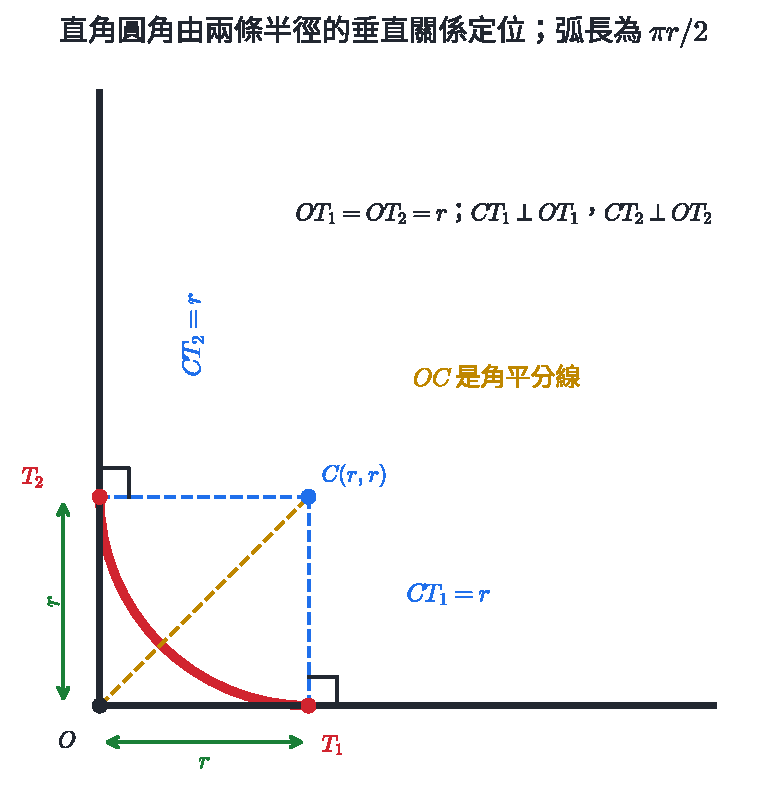
\includegraphics[width=0.84\linewidth,height=\textheight,keepaspectratio,alt={直角圓角的圓心與切點}]{assets/數B3-3-圓角切線幾何.pdf}
\caption{直角圓角的圓心與切點}
\end{figure}

直角頂點設為原點，兩邊沿正 \(x,y\) 軸，圓角半徑為 \(r\)。圓心為 \((r,r)\)，兩切點為 \((r,0)\) 與 \((0,r)\)。圓弧是四分之一圓：

\[
s=r\theta=\frac{\pi r}{2}.
\]

若從 \(r\times r\) 的正方形角落裁去圓角，裁下碎片面積為

\[
r^2-\frac14\pi r^2=r^2\left(1-\frac\pi4\right).
\]

相似圖形若長度倍率為 \(k\)，周長乘 \(|k|\)、面積乘 \(k^2\)。這使設計稿可先以小比例驗證，再按倍率輸出。

\subsection{示範 1｜由圓弧長反求半徑}\label{ux793aux7bc4-1ux7531ux5713ux5f27ux9577ux53cdux6c42ux534aux5f91}

直角圓角的弧長為 \(12\pi\text{ mm}\)，求半徑。

\textbf{解。}

\[
\frac{\pi r}{2}=12\pi\Rightarrow r=24\text{ mm}.
\]

兩切點各離直角頂點 \(24\text{ mm}\)。

\subsection{示範 2｜四個圓角裁下的總面積}\label{ux793aux7bc4-2ux56dbux500bux5713ux89d2ux88c1ux4e0bux7684ux7e3dux9762ux7a4d}

一張矩形卡紙四角都裁成半徑 \(10\text{ mm}\) 的圓角。求四塊碎片總面積。

\textbf{解。} 每塊碎片為正方形減四分之一圓：

\[
10^2-\frac14\pi(10)^2=100-25\pi.
\]

四塊總面積為

\[
4(100-25\pi)=400-100\pi\text{ mm}^2.
\]

\subsection{13.2 分節練習}\label{ux5206ux7bc0ux7df4ux7fd2-12}

\begin{enumerate}
\def\labelenumi{\arabic{enumi}.}
\tightlist
\item
  半徑 \(8\text{ mm}\) 的直角圓角，求弧長。
\item
  直角圓角的圓心為 \((15,15)\)，兩邊為坐標軸。寫出兩切點。
\item
  一個 \(90^\circ\) 圓角的弧長為 \(7\pi\text{ cm}\)，求半徑。
\item
  四個半徑 \(6\text{ mm}\) 的圓角碎片總面積為何？
\item
  一個標誌等比例放大 \(2.5\) 倍。原周長 \(48\text{ cm}\)、面積 \(90\text{ cm}^2\)，求新周長與面積。
\end{enumerate}

\subsection{13.3 分節練習解析}\label{ux5206ux7bc0ux7df4ux7fd2ux89e3ux6790-12}

\begin{enumerate}
\def\labelenumi{\arabic{enumi}.}
\tightlist
\item
  \(s=8(\pi/2)=4\pi\text{ mm}\)。
\item
  切點是 \((15,0)\) 與 \((0,15)\)。
\item
  \(\pi r/2=7\pi\)，得 \(r=14\text{ cm}\)。
\item
  \(4[6^2-(\pi/4)6^2]=144-36\pi\text{ mm}^2\)。
\item
  新周長 \(48(2.5)=120\text{ cm}\)；新面積 \(90(2.5)^2=562.5\text{ cm}^2\)。
\end{enumerate}

\section{14. 代表題與章末分層練習}\label{ux4ee3ux8868ux984cux8207ux7ae0ux672bux5206ux5c64ux7df4ux7fd2}

\subsection{A. 定義與基本操作}\label{a.-ux5b9aux7fa9ux8207ux57faux672cux64cdux4f5c}

\begin{enumerate}
\def\labelenumi{\arabic{enumi}.}
\item
  四邊形 \(ABCD\) 中，化簡
  \[
  \overrightarrow{AB}+\overrightarrow{DA}+\overrightarrow{BC}.
  \]
\item
  已知 \(A(-4,3)\)、\(B(2,-5)\)。

  \begin{enumerate}
  \def\labelenumii{\arabic{enumii}.}
  \tightlist
  \item
    求 \(\overrightarrow{AB}\) 與 \(AB\)；
  \item
    求與 \(\overrightarrow{AB}\) 同向、長度為 \(5\) 的向量。
  \end{enumerate}
\item
  已知 \(\vec a=(2,1)\)、\(\vec b=(1,-2)\)，把 \((7,-4)\) 寫成 \(x\vec a+y\vec b\)。
\item
  \(A(-1,5)\)、\(B(9,0)\)。求滿足 \(AP:PB=3:2\) 的內分點 \(P\)，以及在 \(B\) 外側、滿足 \(AQ:QB=3:2\) 的外分點 \(Q\)。
\end{enumerate}

\subsection{B. 內積、投影與直線}\label{b.-ux5167ux7a4dux6295ux5f71ux8207ux76f4ux7dda}

\begin{enumerate}
\def\labelenumi{\arabic{enumi}.}
\setcounter{enumi}{4}
\item
  三角形頂點為 \(A(1,1)\)、\(B(5,3)\)、\(C(0,3)\)。判斷 \(\angle BAC\) 為銳角、直角或鈍角，並求其餘弦。
\item
  已知 \(|\vec a|=4\)、\(|\vec b|=3\)、\(\vec a\cdot\vec b=-6\)，求 \(|2\vec a+\vec b|\)。
\item
  把 \(\vec p=(7,1)\) 分解成平行於 \(\vec d=(2,-1)\) 與垂直於 \(\vec d\) 的分量。
\item
  直線 \(L\) 通過 \(A(1,2)\)，方向向量為 \((3,1)\)。求 \(P(5,7)\) 在 \(L\) 上的投影點 \(H\) 與距離 \(PH\)。
\item
  求通過 \(P(-2,4)\) 且與直線 \(3x-4y+7=0\) 平行的直線方程式。
\end{enumerate}

\subsection{C. 比例與設計模型}\label{c.-ux6bd4ux4f8bux8207ux8a2dux8a08ux6a21ux578b}

\begin{enumerate}
\def\labelenumi{\arabic{enumi}.}
\setcounter{enumi}{9}
\item
  一個高 \(4.5\text{ m}\) 的物體距眼睛 \(12\text{ m}\)，畫面距眼睛 \(3\text{ m}\)。求物體在畫面上的高度。若物體再遠離眼睛到 \(18\text{ m}\)，畫面高度變為多少？
\item
  A0 面積為 \(1\text{ m}^2\)。求 A6 面積，以平方公分表示；並求 A3 與 A6 的面積比。
\item
  一個直角圓角弧長為 \(9\pi\text{ mm}\)。求圓角半徑，以及四角都作相同圓角時裁下的總面積。
\end{enumerate}

\subsection{D. 跨節整合}\label{d.-ux8de8ux7bc0ux6574ux5408}

\begin{enumerate}
\def\labelenumi{\arabic{enumi}.}
\setcounter{enumi}{12}
\tightlist
\item
  一條河寬 \(240\text{ m}\)，水流向東 \(3\text{ m/s}\)。船相對水面的速率為 \(5\text{ m/s}\)，希望從南岸 \(A\) 到正北方對岸 \(B\)。

  \begin{enumerate}
  \def\labelenumii{\arabic{enumii}.}
  \tightlist
  \item
    取東、北為正向，求船相對水面的速度向量；
  \item
    求船相對河岸的速度與渡河時間；
  \item
    航程中點 \(M\) 的坐標為何？令 \(A=(0,0)\)。
  \end{enumerate}
\item
  \(A(-2,1)\)、\(B(8,6)\)，點 \(P\) 內分 \(AB\) 且 \(AP:PB=2:3\)。直線 \(L\) 通過 \(P\)，方向向量為 \(\overrightarrow{AB}\)。點 \(C(4,8)\)。

  \begin{enumerate}
  \def\labelenumii{\arabic{enumii}.}
  \tightlist
  \item
    求 \(P\)；
  \item
    求 \(C\) 在 \(L\) 上的投影點 \(H\)；
  \item
    求 \(C\) 到 \(L\) 的距離；
  \item
    寫出 \(L\) 的一般式方程式。
  \end{enumerate}
\item
  建築物立面寬 \(18\text{ m}\)、高 \(12\text{ m}\)，距觀察者 \(30\text{ m}\)；畫面距觀察者 \(5\text{ m}\)。設計師要把畫面上的立面等比例印在 A 系列紙上，並讓印刷寬度為 A4 短邊 \(210\text{ mm}\)。

  \begin{enumerate}
  \def\labelenumii{\arabic{enumii}.}
  \tightlist
  \item
    求建築物在畫面上的寬與高；
  \item
    求從畫面到印刷稿的縮放倍率；
  \item
    求印刷高度；
  \item
    求印刷立面占用面積。
  \end{enumerate}
\item
  一個黃金矩形的短邊為 \(20\text{ cm}\)。設計師切去一個 \(20\times20\) 的正方形，並把剩餘矩形等比例縮小 \(1/2\)，其四角各裁成半徑 \(2\text{ cm}\) 的圓角。

  \begin{enumerate}
  \def\labelenumii{\arabic{enumii}.}
  \tightlist
  \item
    求原黃金矩形長邊；
  \item
    求剩餘矩形縮小後的長與寬；
  \item
    求四段圓角弧長總和；
  \item
    求裁去四角後的面積。
  \end{enumerate}
\end{enumerate}

\section{15. 章末練習完整詳解}\label{ux7ae0ux672bux7df4ux7fd2ux5b8cux6574ux8a73ux89e3}

\subsection{第 1 題}\label{ux7b2c-1-ux984c}

先交換次序，使端點首尾相接：

\[
\overrightarrow{DA}+\overrightarrow{AB}+\overrightarrow{BC}
=\overrightarrow{DB}+\overrightarrow{BC}
=\overrightarrow{DC}.
\]

\subsection{第 2 題}\label{ux7b2c-2-ux984c}

\begin{enumerate}
\def\labelenumi{\arabic{enumi}.}
\tightlist
\item
  終點減起點：
  \[
  \overrightarrow{AB}=(2-(-4),-5-3)=(6,-8),
  \]
  \[
  AB=\sqrt{6^2+(-8)^2}=10.
  \]
\item
  單位同向向量為 \((6,-8)/10=(3/5,-4/5)\)。長度為 \(5\) 的同向向量是
  \[
  5\left(\frac35,-\frac45\right)=(3,-4).
  \]
\end{enumerate}

\subsection{第 3 題}\label{ux7b2c-3-ux984c}

\[
x(2,1)+y(1,-2)=(2x+y,x-2y)=(7,-4).
\]

解聯立

\[
\begin{cases}2x+y=7,\\x-2y=-4,\end{cases}
\]

由第一式 \(y=7-2x\)，代入第二式得 \(5x=10\)，所以

\[
x=2,\qquad y=3.
\]

\subsection{第 4 題}\label{ux7b2c-4-ux984c}

內分點使用權重和：

\[
P=\frac{2A+3B}{5}
=\left(\frac{-2+27}{5},\frac{10}{5}\right)=(5,2).
\]

外分點在 \(B\) 外側，使用權重差：

\[
Q=\frac{3B-2A}{3-2}
=(27,0)-(-2,10)=(29,-10).
\]

檢查 \(AQ=15\sqrt5\)、\(QB=10\sqrt5\)，比例為 \(3:2\)。

\subsection{第 5 題}\label{ux7b2c-5-ux984c}

由 \(A\) 出發的兩向量為

\[
\overrightarrow{AB}=(4,2),\qquad \overrightarrow{AC}=(-1,2).
\]

\[
\overrightarrow{AB}\cdot\overrightarrow{AC}=-4+4=0.
\]

所以 \(\angle BAC=90^\circ\)，其餘弦為 \(0\)。

\subsection{第 6 題}\label{ux7b2c-6-ux984c}

\[
|2\vec a+\vec b|^2
=4|\vec a|^2+4\vec a\cdot\vec b+|\vec b|^2.
\]

代入得到

\[
4(16)+4(-6)+9=49.
\]

因此 \(|2\vec a+\vec b|=7\)。

\subsection{第 7 題}\label{ux7b2c-7-ux984c}

平行分量為

\[
\vec v=\operatorname{proj}_{\vec d}\vec p
=\frac{(7,1)\cdot(2,-1)}{2^2+(-1)^2}(2,-1)
=\frac{13}{5}(2,-1)
=\left(\frac{26}{5},-\frac{13}{5}\right).
\]

垂直分量為

\[
\vec u=\vec p-\vec v
=\left(\frac95,\frac{18}{5}\right).
\]

檢查 \(\vec u\cdot\vec d=18/5-18/5=0\)，且 \(\vec u+\vec v=(7,1)\)。

\subsection{第 8 題}\label{ux7b2c-8-ux984c}

\(\overrightarrow{AP}=(4,5)\)、\(\vec d=(3,1)\)。投影係數為

\[
t=\frac{(4,5)\cdot(3,1)}{3^2+1^2}=\frac{17}{10}.
\]

所以

\[
H=A+t\vec d
=\left(1+\frac{51}{10},2+\frac{17}{10}\right)
=\left(\frac{61}{10},\frac{37}{10}\right).
\]

\[
\overrightarrow{HP}=\left(-\frac{11}{10},\frac{33}{10}\right),
\]

\[
PH=\frac{11\sqrt{10}}{10}.
\]

\subsection{第 9 題}\label{ux7b2c-9-ux984c}

與已知直線平行的直線可使用同一個法向量 \((3,-4)\)：

\[
3(x+2)-4(y-4)=0.
\]

整理得

\[
3x-4y+22=0.
\]

\subsection{第 10 題}\label{ux7b2c-10-ux984c}

物體距眼睛 \(12\text{ m}\) 時，透視倍率為 \(3/12=1/4\)：

\[
h_1=4.5\cdot\frac14=1.125\text{ m}.
\]

距離改成 \(18\text{ m}\) 時，倍率為 \(3/18=1/6\)：

\[
h_2=4.5\cdot\frac16=0.75\text{ m}.
\]

物體變遠後，畫面高度由 \(1.125\) 降為 \(0.75\)，比例為 \(2/3\)，與距離反比一致。

\subsection{第 11 題}\label{ux7b2c-11-ux984c}

A6 經六次對半裁切：

\[
A_6=2^{-6}\text{ m}^2=\frac1{64}\text{ m}^2.
\]

換成平方公分：

\[
\frac{10000}{64}=156.25\text{ cm}^2.
\]

A3 到 A6 相差三次裁切，所以

\[
A3:A6=2^3:1=8:1.
\]

\subsection{第 12 題}\label{ux7b2c-12-ux984c}

四分之一圓弧長為 \(\pi r/2\)：

\[
\frac{\pi r}{2}=9\pi\Rightarrow r=18\text{ mm}.
\]

每角碎片面積為

\[
18^2-\frac14\pi(18)^2=324-81\pi.
\]

四角總面積為

\[
1296-324\pi\text{ mm}^2.
\]

\subsection{第 13 題｜船速、向量合成與中點}\label{ux7b2c-13-ux984cux8239ux901fux5411ux91cfux5408ux6210ux8207ux4e2dux9ede}

\begin{enumerate}
\def\labelenumi{\arabic{enumi}.}
\tightlist
\item
  為抵銷向東 \(3\text{ m/s}\) 的水流，船相對水面的東西分量要向西 \(3\text{ m/s}\)。船速大小為 \(5\)，北向分量設為 \(v\)：
  \[
  (-3)^2+v^2=5^2\Rightarrow v=4.
  \]
  因需向北渡河，取正值，所以船相對水面速度為 \((-3,4)\text{ m/s}\)。
\item
  加上水流 \((3,0)\)：
  \[
  \vec v_{\text{岸}}=(-3,4)+(3,0)=(0,4)\text{ m/s}.
  \]
  渡河時間
  \[
  t=\frac{240}{4}=60\text{ s}.
  \]
\item
  令 \(A=(0,0)\)，則 \(B=(0,240)\)。中點
  \[
  M=\frac{A+B}{2}=(0,120).
  \]
  地面軌跡是正北直線，符合東西分量已抵銷。
\end{enumerate}

\subsection{第 14 題｜分點、投影、距離與直線}\label{ux7b2c-14-ux984cux5206ux9edeux6295ux5f71ux8dddux96e2ux8207ux76f4ux7dda}

\begin{enumerate}
\def\labelenumi{\arabic{enumi}.}
\tightlist
\item
  \(AP:PB=2:3\)：
  \[
  P=\frac{3A+2B}{5}
  =\left(\frac{-6+16}{5},\frac{3+12}{5}\right)=(2,3).
  \]
\item
  \(\vec d=\overrightarrow{AB}=(10,5)\)，可約成 \((2,1)\)。\(\overrightarrow{PC}=(2,5)\)。投影係數
  \[
  t=\frac{(2,5)\cdot(2,1)}{2^2+1^2}=\frac95.
  \]
  因此
  \[
  H=P+\frac95(2,1)=\left(\frac{28}{5},\frac{24}{5}\right).
  \]
\item
  \[
  \overrightarrow{HC}
  =\left(-\frac85,\frac{16}{5}\right),
  \]
  所以
  \[
  CH=\frac{8\sqrt5}{5}.
  \]
\item
  \((2,1)\) 的一個法向量是 \((1,-2)\)。通過 \(P(2,3)\)：
  \[
  (x-2)-2(y-3)=0
  \Rightarrow x-2y+4=0.
  \]
\end{enumerate}

\subsection{第 15 題｜透視比例與印刷縮放}\label{ux7b2c-15-ux984cux900fux8996ux6bd4ux4f8bux8207ux5370ux5237ux7e2eux653e}

\begin{enumerate}
\def\labelenumi{\arabic{enumi}.}
\tightlist
\item
  畫面倍率為 \(5/30=1/6\)，所以
  \[
  w=18\cdot\frac16=3\text{ m},\qquad
  h=12\cdot\frac16=2\text{ m}.
  \]
\item
  把畫面寬 \(3\text{ m}=3000\text{ mm}\) 縮成 \(210\text{ mm}\)：
  \[
  r=\frac{210}{3000}=0.07.
  \]
\item
  印刷高度
  \[
  2000(0.07)=140\text{ mm}.
  \]
\item
  印刷面積
  \[
  210\cdot140=29400\text{ mm}^2=294\text{ cm}^2.
  \]
  寬高比 \(210:140=3:2\)，與建築物 \(18:12\) 相同。
\end{enumerate}

\subsection{第 16 題｜黃金比例、縮放與圓角}\label{ux7b2c-16-ux984cux9ec3ux91d1ux6bd4ux4f8bux7e2eux653eux8207ux5713ux89d2}

\begin{enumerate}
\def\labelenumi{\arabic{enumi}.}
\tightlist
\item
  原矩形長邊
  \[
  L=20\varphi=10(1+\sqrt5)\text{ cm}.
  \]
\item
  切去 \(20\times20\) 正方形後，剩餘矩形兩邊為 \(20\) 與
  \[
  20\varphi-20=20(\varphi-1)=\frac{20}{\varphi}.
  \]
  縮小 \(1/2\) 後，長、寬分別為
  \[
  10\text{ cm},\qquad \frac{10}{\varphi}=10(\varphi-1)\text{ cm}.
  \]
\item
  每段圓角為四分之一圓，半徑 \(2\)：
  \[
  4\left(\frac{\pi(2)}2\right)=4\pi\text{ cm}.
  \]
\item
  圓角前面積
  \[
  A_0=10\cdot\frac{10}{\varphi}=\frac{100}{\varphi}.
  \]
  每角裁下 \(2^2-(\pi/4)2^2=4-\pi\)，四角共 \(16-4\pi\)。因此
  \[
  A=\frac{100}{\varphi}-16+4\pi\text{ cm}^2.
  \]
  因 \(100/\varphi\approx61.80\)，結果約為 \(58.37\text{ cm}^2\)，為正且小於圓角前面積。
\end{enumerate}

\section{16. 核心整理}\label{ux6838ux5fc3ux6574ux7406}

\subsection{向量表示與比例}\label{ux5411ux91cfux8868ux793aux8207ux6bd4ux4f8b}

{\def\LTcaptype{none} % do not increment counter
\begin{longtable}[]{@{}
  >{\raggedright\arraybackslash}p{(\linewidth - 4\tabcolsep) * \real{0.3333}}
  >{\raggedright\arraybackslash}p{(\linewidth - 4\tabcolsep) * \real{0.3333}}
  >{\raggedright\arraybackslash}p{(\linewidth - 4\tabcolsep) * \real{0.3333}}@{}}
\toprule\noalign{}
\begin{minipage}[b]{\linewidth}\raggedright
問題
\end{minipage} & \begin{minipage}[b]{\linewidth}\raggedright
公式
\end{minipage} & \begin{minipage}[b]{\linewidth}\raggedright
條件與幾何意義
\end{minipage} \\
\midrule\noalign{}
\endhead
\bottomrule\noalign{}
\endlastfoot
由兩點求向量 & \(\overrightarrow{AB}=(x_B-x_A,y_B-y_A)\) & 終點減起點，方向由 \(A\) 到 \(B\) \\
向量長度 & \(|(u,v)|=\sqrt{u^2+v^2}\) & 畢氏定理 \\
平行判定 & \(a_1b_2-a_2b_1=0\) & 兩向量皆非零時可寫成倍數關係 \\
線性組合 & \(\vec p=x\vec a+y\vec b\) & \(\vec a,\vec b\) 不平行時表示唯一 \\
內分點 & \(P=(nA+mB)/(m+n)\) & \(AP:PB=m:n\)，\(P\) 在 \(A,B\) 之間 \\
外分點 & \(Q=(mB-nA)/(m-n)\) & \(AQ:QB=m:n\)，點的順序先確定 \\
縮放平移 & \(P'=rP+\vec t\) & 長度倍率 \(|r|\)，面積倍率 \(r^2\) \\
\end{longtable}
}

\subsection{內積、投影與直線}\label{ux5167ux7a4dux6295ux5f71ux8207ux76f4ux7dda}

{\def\LTcaptype{none} % do not increment counter
\begin{longtable}[]{@{}
  >{\raggedright\arraybackslash}p{(\linewidth - 4\tabcolsep) * \real{0.3333}}
  >{\raggedright\arraybackslash}p{(\linewidth - 4\tabcolsep) * \real{0.3333}}
  >{\raggedright\arraybackslash}p{(\linewidth - 4\tabcolsep) * \real{0.3333}}@{}}
\toprule\noalign{}
\begin{minipage}[b]{\linewidth}\raggedright
問題
\end{minipage} & \begin{minipage}[b]{\linewidth}\raggedright
公式
\end{minipage} & \begin{minipage}[b]{\linewidth}\raggedright
條件與幾何意義
\end{minipage} \\
\midrule\noalign{}
\endhead
\bottomrule\noalign{}
\endlastfoot
內積 & \(\vec a\cdot\vec b=|a||b|\cos\theta=a_1b_1+a_2b_2\) & 共同起點夾角 \(0^\circ\le\theta\le180^\circ\) \\
垂直 & \(\vec a\cdot\vec b=0\) & 兩向量非零 \\
功 & \(W=\vec F\cdot\vec s\) & 計入力沿位移方向的分量，單位 J \\
長度展開 & \(|a\pm b|^2=|a|^2\pm2a\cdot b+|b|^2\) & 用內積處理對角線與組合向量 \\
正射影 & \(\operatorname{proj}_{b}a=(a\cdot b/|b|^2)b\) & \(b\ne0\) \\
投影點 & \(H=A+\operatorname{proj}_{d}\overrightarrow{AP}\) & \(A\) 在直線上，\(d\) 為方向向量 \\
法向量直線 & \(a(x-x_0)+b(y-y_0)=0\) & \((a,b)\) 垂直於直線 \\
\end{longtable}
}

\subsection{透視與設計比例}\label{ux900fux8996ux8207ux8a2dux8a08ux6bd4ux4f8b}

{\def\LTcaptype{none} % do not increment counter
\begin{longtable}[]{@{}
  >{\raggedright\arraybackslash}p{(\linewidth - 4\tabcolsep) * \real{0.3333}}
  >{\raggedright\arraybackslash}p{(\linewidth - 4\tabcolsep) * \real{0.3333}}
  >{\raggedright\arraybackslash}p{(\linewidth - 4\tabcolsep) * \real{0.3333}}@{}}
\toprule\noalign{}
\begin{minipage}[b]{\linewidth}\raggedright
模型
\end{minipage} & \begin{minipage}[b]{\linewidth}\raggedright
核心關係
\end{minipage} & \begin{minipage}[b]{\linewidth}\raggedright
用途與範圍
\end{minipage} \\
\midrule\noalign{}
\endhead
\bottomrule\noalign{}
\endlastfoot
單點透視 & \(h/H=d/D\) & 直線投影與同深度平面的尺寸比例 \\
A 系列紙張 & 長寬比 \(\sqrt2:1\)，A\(n\) 面積 \(2^{-n}\text{ m}^2\) & 對半裁切後仍相似；實際毫米數含取整 \\
黃金分割 & \(\varphi=(1+\sqrt5)/2\)，\(\varphi^2=\varphi+1\) & 線段分割、矩形自相似、費氏相鄰比 \\
直角圓角 & 圓心 \((r,r)\)，弧長 \(\pi r/2\) & 半徑垂直切線，圓心在角平分線上 \\
\end{longtable}
}

完成向量題時，先畫出起點、終點與箭頭，再轉成坐標；完成投影題時，先標出平行方向與垂直剩餘分量；完成比例題時，先寫出對應長度與相似比。圖中的方向、點序與倍率會直接決定公式中的正負號與分母。


\end{document}
